%% Tesseract: Journal Extension (ACM TSAS) - REVISION 1, clean copy (no colors)
%% Extended from: "Tesseract: Unfolding Navigable Graph Representations from Low-Semantic Floor Plans"
%%
%% Colour code (see revision_macros.tex and paper/README.md):
%%   \rone{}  Reviewer 1 (blue)   \rtwo{}   Reviewer 2 (green)
%%   \rthree{} Reviewer 3 (purple) \rall{}  editor / multiple (vermilion)
%%   \rdel{}  deletions (struck out here, absent in the clean copy)
%% Uncolored new text = editorial improvements not tied to a reviewer.
%% Float discipline: every figure/table is sourced immediately at its first
%% reference with [t] placement.

\documentclass[manuscript,screen,review]{acmart}

% BibTeX logo
\AtBeginDocument{%
  \providecommand\BibTeX{{Bib\TeX}}}

% Packages
\usepackage{graphicx}
\usepackage{booktabs}
\usepackage{multirow}
\usepackage{algorithm}
\usepackage{algorithmic}
\usepackage{xcolor}
\usepackage{subcaption}
\usepackage{tikz}
\usetikzlibrary{positioning}
% ============================================================================
% revision_macros.tex - per-reviewer revision markup (TSAS revision round 1)
%
% Usage in main_revision_1.tex:
%   \rone{new text addressing Reviewer 1}
%   \rtwo{...Reviewer 2...}   \rthree{...Reviewer 3...}
%   \rall{...editor / multiple reviewers...}
%   \rdel{deleted text}       (struck out in coloured mode, GONE in clean mode)
%
% All commands are \DeclareRobustCommand, so they work inside \caption{},
% \section{}, table cells, and footnotes.
%
% The clean copy is generated by make_clean.sh, which flips \revcolortrue
% to \revcolorfalse - do not edit main_revision_1_clean.tex by hand.
% ============================================================================
\makeatletter
\@ifpackageloaded{xcolor}{}{\usepackage{xcolor}}
\@ifpackageloaded{ulem}{}{\usepackage[normalem]{ulem}}
\makeatother

\definecolor{RevOneCol}{RGB}{0,84,159}     % Reviewer 1 - blue
\definecolor{RevTwoCol}{RGB}{0,122,94}     % Reviewer 2 - green
\definecolor{RevThreeCol}{RGB}{118,42,131} % Reviewer 3 - purple
\definecolor{RevAllCol}{RGB}{178,58,0}     % Editor / multiple reviewers - vermilion

\newif\ifrevcolor
\revcolortrue

\DeclareRobustCommand{\rone}[1]{\ifrevcolor\textcolor{RevOneCol}{#1}\else#1\fi}
\DeclareRobustCommand{\rtwo}[1]{\ifrevcolor\textcolor{RevTwoCol}{#1}\else#1\fi}
\DeclareRobustCommand{\rthree}[1]{\ifrevcolor\textcolor{RevThreeCol}{#1}\else#1\fi}
\DeclareRobustCommand{\rall}[1]{\ifrevcolor\textcolor{RevAllCol}{#1}\else#1\fi}
\DeclareRobustCommand{\rdel}[1]{\ifrevcolor{\color{gray}\sout{#1}}\fi}
\revcolorfalse   % colors disabled in this clean copy

% Float discipline: floats stay in their section and place eagerly.
\usepackage[section]{placeins}
\renewcommand{\topfraction}{0.9}
\renewcommand{\bottomfraction}{0.6}
\renewcommand{\textfraction}{0.07}
\renewcommand{\floatpagefraction}{0.75}
\setcounter{topnumber}{3}
\setcounter{totalnumber}{5}

% Custom commands
\newcommand{\tesseract}{\textsc{Tesseract}}
\newcommand{\eg}{\textit{e.g.}}
\newcommand{\ie}{\textit{i.e.}}
\newcommand{\etal}{\textit{et al.}}

\begin{document}

% ==============================================================================
% TITLE
% ==============================================================================
\title[Tesseract: Indoor Graph Maps from Low-Semantic Floor Plans]{%
Tesseract: Generating Indoor Graph Maps from Large-Scale Low-Semantic Floor Plans}

% ==============================================================================
% AUTHORS
% ==============================================================================
\author{Yaqoob Ansari}
\affiliation{%
  \institution{Carnegie Mellon University}
  \city{Pittsburgh}
  \state{PA}
  \country{USA}
}
\email{yansari@andrew.cmu.edu}

\author{Eduardo Feo Flushing}
\affiliation{%
  \institution{Carnegie Mellon University}
  \city{Pittsburgh}
  \state{PA}
  \country{USA}
}
\email{efeoflus@andrew.cmu.edu}

\author{Khaled A. Harras}
\affiliation{%
  \institution{Carnegie Mellon University}
  \city{Pittsburgh}
  \state{PA}
  \country{USA}
}
\email{kharras@andrew.cmu.edu}

\renewcommand{\shortauthors}{Ansari et al.}

% ==============================================================================
% ABSTRACT
% ==============================================================================
\begin{abstract}
Indoor navigation and spatial reasoning require structured representations of building layouts. Converting architectural floorplans into machine-readable navigable graphs remains difficult because visual annotations carry no explicit topological connectivity. We present \tesseract{}, an end-to-end system that transforms annotated building floorplans into multi-floor navigable graph representations. The pipeline detects and interprets text labels to seed rooms, corridors, outdoor areas, and vertical transition elements. It then segments the drawing with flood fill, places spatial subnodes with distance-transform guidance, and detects doors with a type-aware classifier that distinguishes room-to-corridor, room-to-room, and exit doors. Graph construction uses room-family funneling, \rone{a construction with a proven guarantee that every room point reaches every room door while the number of intra-room edges stays linear in the subnode count}. \rall{For multi-floor buildings, \tesseract{} infers vertical correspondences automatically. A registration stage aligns adjacent floor drawings using wall evidence and a drawing-scale prior, and a globally optimal assignment with a rejection option pairs stairs and elevators across floors while leaving terminating shafts unmatched. Hand-written mappings remain available as an optional override, and floor indices are read from a filename convention.} We evaluate the system with degradation studies, ablations, an objective route-fidelity reference based on free-space geodesics, and a quantitative baseline comparison. Graph routes stay within 4.7\% of the shortest walkable paths on the primary evaluation floor, and pruning removes 59\% of nodes and 82\% of edges with no measured route inflation.
\end{abstract}

% ==============================================================================
% CCS CONCEPTS
% ==============================================================================
\begin{CCSXML}
<ccs2012>
 <concept>
  <concept_id>10002951.10003260</concept_id>
  <concept_desc>Information systems~Geographic information systems</concept_desc>
  <concept_significance>500</concept_significance>
 </concept>
 <concept>
  <concept_id>10010147.10010257</concept_id>
  <concept_desc>Computing methodologies~Computer vision</concept_desc>
  <concept_significance>500</concept_significance>
 </concept>
 <concept>
  <concept_id>10003752.10003753.10003754</concept_id>
  <concept_desc>Theory of computation~Graph algorithms analysis</concept_desc>
  <concept_significance>300</concept_significance>
 </concept>
</ccs2012>
\end{CCSXML}

\ccsdesc[500]{Information systems~Geographic information systems}
\ccsdesc[500]{Computing methodologies~Computer vision}
\ccsdesc[300]{Theory of computation~Graph algorithms analysis}

% ==============================================================================
% KEYWORDS
% ==============================================================================
\keywords{floorplan parsing, indoor navigation, spatial graphs, semantic mapping, door detection, multi-floor connectivity, building information extraction, graph construction}

\maketitle

% ==============================================================================
% 1. INTRODUCTION
% ==============================================================================
\section{Introduction}
\label{sec:introduction}

Indoor navigation depends on structured representations of architectural layouts. Robotic path planning and building accessibility analysis share the same dependency. Outdoor navigation benefits from mature geographic information systems and standardized road network graphs. Indoor environments offer no such standard. Buildings exhibit complex multi-room topologies, vertical connectivity through stairs and elevators, and semantic distinctions between navigable corridors, restricted areas, and transition zones. Converting architectural floorplans, the primary documentation of building layouts, into machine-readable navigable graphs therefore remains a significant technical challenge.

Legacy floorplans dominate the available documentation. Existing approaches to indoor map generation often require manual annotation, assume access to Building Information Models (BIM), or rely on sensor-based simultaneous localization and mapping (SLAM). Vast repositories of institutional, commercial, and residential floorplans instead exist as raster images with minimal semantic markup. These drawings contain text annotations identifying rooms and spaces, standard symbols for doors, and dark strokes for walls. They lack the structured connectivity information that navigation applications require.

This manuscript substantially extends our prior conference publication~\cite{tesseract_conference}, which introduced the core single-floor parsing pipeline. \rthree{The extension centers on two contributions. First, a multi-floor graph construction module that infers vertical correspondences between floors automatically, registers adjacent floor drawings into a common frame, and merges per-floor graphs into a unified building representation. Second, a room-family representation with distance-transform subnodes and a funneling construction whose connectivity guarantee we state and prove. The remaining additions support these two contributions:}
\begin{itemize}
    \item \rall{Automatic inter-floor transition matching, formulated as wall-evidence registration followed by optimal assignment with a rejection option, with hand-written mappings retained as an override.}
    \item \rone{A proven funneling guarantee, complete intra-room connectivity at linear intra-room edge cost, validated by a three-way ablation against dense and single-node room encodings.}
    \item \rthree{A deepened evaluation of type-aware door connectivity, including degradation studies that quantify how detector errors propagate to graph connectivity.}
    \item \rall{An expanded experimental methodology covering text accuracy, corridor density, pruning ablations, an objective route-fidelity reference, downstream navigation tasks, and a quantitative baseline.}
\end{itemize}

\tesseract{} operates as a modular pipeline. Given raster floorplan images with text annotations and standard architectural conventions, it produces typed, attributed graphs in which nodes represent spatial regions and edges encode traversability with geometric distance weights. Text detection and semantic interpretation identify labeled regions. Flood-fill segmentation with subnode placement encodes spatial extent. Door detection and classification establish connectivity. Graph construction with pruning produces well-conditioned outputs for pathfinding algorithms.

A hierarchical room representation underlies the graph construction. Rooms in architectural floorplans may span large areas with complex shapes, yet navigation requires fine-grained spatial encoding. Each semantic room therefore contains a designated main node and multiple subnodes sampled on a hexagonal grid within the room boundary. \rone{Room-family funneling connects each family through a shortest-path tree rooted at the main node, plus a single shortcut edge from each door to its closest family node. This construction guarantees that every subnode reaches every room door while spending only linearly many intra-room edges. Subnodes adjacent to a door exit directly rather than detouring through the room center.}

\rall{Multi-floor construction no longer depends on hand-written correspondences. The system registers adjacent floor drawings using wall-mask evidence and a drawing-scale prior bootstrapped from detected door widths. It then solves a global assignment problem over the detected stairs and elevators, with an explicit rejection option so that shafts without a counterpart remain unmatched. Validation rules that previously checked a human's input now verify the machine's answer. Two elements remain metadata-assisted by design. Floor indices are read from a filename convention, and a hand-written mapping file can override the inferred correspondence.}

The remainder of this paper is organized as follows. Section~\ref{sec:related_work} surveys related work. Section~\ref{sec:problem} defines the problem and output schema. Section~\ref{sec:system_overview} presents the system architecture. Sections~\ref{sec:text_detection}--\ref{sec:multi_floor} detail the pipeline components. Section~\ref{sec:experiments} presents the experimental evaluation. Section~\ref{sec:discussion} discusses limitations. Section~\ref{sec:conclusion} concludes.

% ==============================================================================
% 2. RELATED WORK
% ==============================================================================
\section{Related Work}
\label{sec:related_work}

\paragraph{Floorplan Recognition and Parsing.}
Learned floorplan parsing has advanced rapidly. Raster-to-vector conversion recovers junction and wall structure from rasterized drawings~\cite{raster_to_vector}, CubiCasa5k provides a large annotated corpus with a multi-task parsing network~\cite{cubicasa}, and room-boundary-aware networks improve wall and opening recovery~\cite{floorplan_parsing_deep}. FloorNet reconstructs floorplans from RGBD scans rather than drawings~\cite{floornet}. These systems target geometric reconstruction. They recover walls, rooms, and openings, but they do not produce navigable graphs with typed nodes, traversability edges, or vertical connectivity. \tesseract{} consumes the same class of raster inputs and outputs a routing-ready representation directly.

\paragraph{Indoor Mapping and Localization.}
Sensor-driven pipelines build maps by traversing the building. SLAM systems produce metric maps from robot or handheld sensing~\cite{slam_survey}, and WiFi fingerprinting supports localization once a signal survey exists~\cite{wifi_fingerprinting}. Both require physical access, instrumentation, and survey effort per building~\cite{indoor_navigation_survey}. Floorplan-based extraction sidesteps deployment cost entirely because the drawing already exists, which makes it attractive for large legacy portfolios.

\paragraph{Graph-Based Spatial Representations.}
Navigation systems consume topological graphs rather than raster maps. IndoorGML standardizes indoor spaces as cellular graphs with connectivity relations~\cite{indoorgml}, and classic shortest-path algorithms operate directly on weighted graphs~\cite{dijkstra, astar}. Wayfinding research further motivates typed nodes because route semantics matter to users~\cite{wayfinding}, and accessibility analysis requires explicit transition elements~\cite{accessibility_analysis}. Our output schema follows this line. Nodes are typed, edges carry geometric weights, and stairs and elevators are first-class objects.

\paragraph{Scene Text Detection and Recognition.}
The Character Region Awareness for Text (CRAFT) detector predicts character-level region and affinity heatmaps and achieves strong accuracy on scene text benchmarks~\cite{craft}. EAST offers an efficient single-stage alternative~\cite{east}. For recognition, convolutional recurrent architectures with Connectionist Temporal Classification (CTC) decoding remain the standard for unconstrained strings~\cite{crnn, ctc}. We adopt CRAFT for detection and a CTC-based recognizer for interpretation because floorplan labels are short, sparse, and often rotated.

\paragraph{Architectural Element Detection.}
Door symbols are small, stylized, and easily confused with other arcs. We build on Faster R-CNN~\cite{faster_rcnn} with a ResNet backbone and feature pyramid~\cite{resnet, fpn}, fine-tuned on floorplan door symbols. Generic detectors transfer poorly to drawings without such fine-tuning because the symbol distribution differs sharply from natural images.

\paragraph{Multi-Floor Building Representations.}
BIM and IFC models encode complete vertical structure~\cite{bim_survey, ifc}, but they exist mainly for recent construction and demand heavyweight tooling. Lightweight navigation graphs derived from per-floor drawings must instead recover vertical connectivity after the fact. To our knowledge, automatic inference of stair and elevator correspondences from raster floor drawings alone has not been addressed, and this gap motivates the matching module of Section~\ref{sec:multi_floor}.

% ==============================================================================
% 3. PROBLEM FORMULATION
% ==============================================================================
\section{Problem Setting and Output Schema}
\label{sec:problem}

\subsection{Input Assumptions}
\label{subsec:input}

\rone{The underlying representation is raster image space, and the pixel is the atomic unit of every pipeline stage.} \tesseract{} accepts floorplan images satisfying the following assumptions:

\begin{enumerate}
    \item \textbf{Text annotations}. Rooms and spaces carry text labels, and \rtwo{semantic classes are seeded exclusively by these labels rather than by fill colors}. Table~\ref{tab:vocabulary} lists the recognized vocabulary.
    \item \textbf{Architectural symbols}. Doors follow standard drafting conventions with arc symbols indicating swing direction.
    \item \textbf{Wall encoding}. Walls appear as dark strokes recoverable by intensity thresholding.
    \item \textbf{Floor naming}. For multi-floor processing, filenames encode floor identity, with FF, SF, and TF denoting the first, second, and third floors, B1 and B2 denoting basements, and numeric prefixes mapping directly.
\end{enumerate}

\begin{table}[!htbp]
\centering
\caption{\rtwo{Label vocabulary. Interpretation is case-insensitive with single-edit fuzzy matching, and every semantic class must be present for door classification to proceed.}}
\label{tab:vocabulary}
\begin{tabular}{ll}
\toprule
Label on drawing & Interpreted as \\
\midrule
any numeric token (\eg, 1001) & room, with the number as its name \\
hall, hallway, corridor, passage & corridor region \\
na & outside or non-navigable region \\
stairs, stair, staircase & stairs transition node \\
elev, elevator, lift & elevator transition node \\
\bottomrule
\end{tabular}
\end{table}

\rthree{These assumptions define an explicit operating envelope. The system targets institutional and commercial drawings that follow standard drafting conventions and carry the label vocabulary above. It does not target hand-drawn sketches, sparsely annotated plans, or drawings with non-standard door symbols. A drawing that lacks corridor, outside, or transition labels fails the semantic-class requirement and is rejected rather than silently mis-segmented, and Section~\ref{subsec:text_eval} demonstrates this failure mode on an unlabeled variant of an evaluation floor.}

\subsection{Output Graph Schema}
\label{subsec:output}

The output is a typed, attributed graph $G = (V, E)$ with node set $V = V_{\text{room}} \cup V_{\text{corridor}} \cup V_{\text{outside}} \cup V_{\text{door}} \cup V_{\text{transition}}$.

Each node $v \in V$ carries the following attributes:
\begin{itemize}
    \item \texttt{id}, a unique string identifier
    \item \texttt{type}, one of room, corridor, outside, door, or transition
    \item \texttt{position}, the $(x, y)$ pixel coordinates
    \item \texttt{floor}, an integer floor identifier
    \item \texttt{pixels}, the region's pixel set for area nodes
\end{itemize}

Each edge $e = (u, v) \in E$ carries the following attributes:
\begin{itemize}
    \item \texttt{weight}, the Euclidean distance between node positions
    \item \texttt{distance}, the geometric distance in pixels
    \item \texttt{edge\_type}, which distinguishes intra-floor from inter-floor edges in merged graphs
\end{itemize}

\rtwo{The graph is undirected. An exit door is defined as a door whose two incident regions are an interior space and an outdoor region. One-way restrictions and emergency-only egress are not modeled, and Section~\ref{sec:discussion} lists directional edge attributes as the natural extension.}

For buildings with multiple floors, the merged graph uses floor-prefixed node identifiers such as \texttt{1\_stairs\_1} to ensure uniqueness, and it preserves the original identifier in a node attribute.

\subsection{Downstream Applications}
\label{subsec:applications}

The output graph supports the following tasks:
\begin{itemize}
    \item \textbf{Pathfinding} with Dijkstra or A* over distance weights
    \item \textbf{Accessibility analysis}, including step-free routing over typed transitions
    \item \textbf{Egress analysis} through exit doors
    \item \textbf{Spatial queries} over room adjacency and floor connectivity
    \item \textbf{Integration} through JSON export compatible with GIS tools
\end{itemize}

\rone{Section~\ref{subsec:downstream} validates the first three tasks directly instead of leaving the application claims implicit.}

% ==============================================================================
% 4. SYSTEM OVERVIEW
% ==============================================================================
\section{System Overview}
\label{sec:system_overview}

Figure~\ref{fig:pipeline} illustrates the \tesseract{} pipeline. Processing proceeds through six stages:

\begin{figure}[!htbp]
\centering
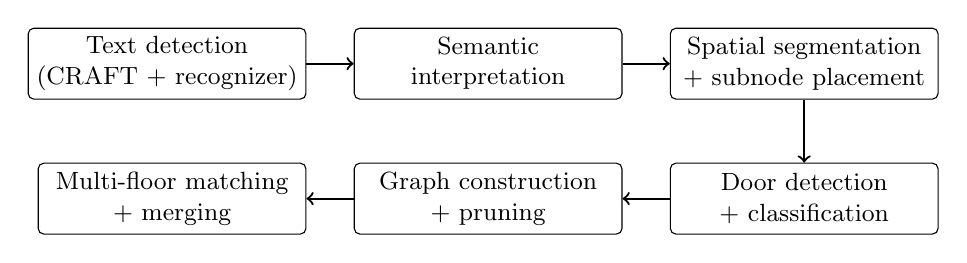
\begin{tikzpicture}[
  stage/.style={draw, rounded corners=2pt, align=center, minimum height=9mm, minimum width=34mm, inner sep=3pt, font=\small},
  arr/.style={->, thick}]
\node[stage] (a) {Text detection\\(CRAFT + recognizer)};
\node[stage, right=6mm of a] (b) {Semantic\\interpretation};
\node[stage, right=6mm of b] (c) {Spatial segmentation\\+ subnode placement};
\node[stage, below=8mm of c] (d) {Door detection\\+ classification};
\node[stage, left=6mm of d] (e) {Graph construction\\+ pruning};
\node[stage, left=6mm of e] (f) {Multi-floor matching\\+ merging};
\draw[arr] (a) -- (b);
\draw[arr] (b) -- (c);
\draw[arr] (c) -- (d);
\draw[arr] (d) -- (e);
\draw[arr] (e) -- (f);
\end{tikzpicture}
\Description{Six pipeline stages connected by arrows.}
\caption{Pipeline architecture. Each single-floor stage feeds the next, and the multi-floor stage consumes the per-floor graphs together with the floor drawings.}
\label{fig:pipeline}
\end{figure}

\begin{enumerate}
    \item \textbf{Text Detection and Recognition} (Section~\ref{sec:text_detection}). CRAFT-based detection followed by CTC-based recognition extracts text annotations.
    \item \textbf{Semantic Interpretation} (Section~\ref{sec:text_detection}). Detected text seeds room labels, corridor markers, outdoor indicators, and transition elements.
    \item \textbf{Spatial Segmentation} (Section~\ref{sec:segmentation}). Flood fill segments the drawing, and distance-transform-guided sampling places subnodes.
    \item \textbf{Door Detection and Classification} (Section~\ref{sec:doors}). Faster R-CNN detects door symbols, and refinement plus classification distinguishes door types.
    \item \textbf{Graph Construction and Pruning} (Section~\ref{sec:graph}). Nodes and edges are assembled and pruned while preserving reachability.
    \item \textbf{Multi-Floor Connectivity} (Section~\ref{sec:multi_floor}). Floor graphs are merged, and transitions are matched across floors automatically.
\end{enumerate}

\paragraph{Timing Characteristics.}
Single-floor processing takes about 52 seconds for a $1946 \times 1574$ image on a standard CPU. Door detection dominates at about 21 seconds, followed by flood-fill segmentation at about 9 seconds. Multi-floor matching and merging add under two seconds. Section~\ref{subsec:timing} gives the full breakdown.

% ==============================================================================
% 5. TEXT DETECTION AND SEMANTIC INTERPRETATION
% ==============================================================================
\section{Text Detection and Semantic Interpretation}
\label{sec:text_detection}

\subsection{Text Region Detection}
\label{subsec:detection}

Text regions are located with the CRAFT detector~\cite{craft}. CRAFT predicts a region score indicating character centers and an affinity score encoding character adjacency, and connected component analysis on the combined heatmap yields word-level boxes. The detector outputs quadrilateral boxes, which accommodates the rotated text common in architectural drawings.

\subsection{Text Recognition}
\label{subsec:recognition}

Detected regions are recognized by a sequence model. \rone{The recognizer combines a Visual Geometry Group (VGG) convolutional feature extractor, a bidirectional Long Short-Term Memory (BiLSTM) sequence encoder, and a Connectionist Temporal Classification (CTC) decoder~\cite{crnn, ctc}.} Each cropped region is normalized before decoding.

\rone{Recognition output is normalized by semantic context rather than by generic spell correction. Tokens are matched against the closed label vocabulary of Table~\ref{tab:vocabulary} with case folding and single-edit fuzzy tolerance. An alphabetic token of three or more characters matches a vocabulary word within Levenshtein distance one, which absorbs single-character OCR confusions such as nna for na. A token within distance one of words from two different classes is rejected as ambiguous. Numeric tokens never fuzzy-match because they are room identifiers, and alphabetic look-alikes inside otherwise numeric tokens are instead mapped to digits, which resolves confusions such as the letter O for the digit zero.}

\subsection{Semantic Interpretation}
\label{sec:interpretation}

The interpretation module classifies recognized strings into the classes of Table~\ref{tab:vocabulary}. Numeric tokens become room identifiers, and the text position seeds the room's main node. Corridor and outside keywords seed region segmentation. Transition keywords produce typed stairs and elevator nodes, which later anchor inter-floor matching. The module outputs a mapping from text regions to semantic types that seeds all subsequent stages.

% ==============================================================================
% 6. SPATIAL SEGMENTATION
% ==============================================================================
\section{Spatial Segmentation and Region Encoding}
\label{sec:segmentation}

\subsection{Wall Mask Extraction}
\label{subsec:masks}

Walls are extracted by intensity thresholding. Near-black pixels form the wall mask, and morphological dilation expands it to separate adjacent regions. \rone{Text strokes also fall below the threshold and therefore enter the wall mask, and we measured them at roughly 9\% of wall ink on the primary evaluation floor. This contamination is harmless during segmentation because flood fill treats glyphs as small obstacles and the dilation buffer dominates. The registration module of Section~\ref{sec:multi_floor}, where wall masks serve as alignment evidence, removes glyphs explicitly by connected-component filtering.}

\subsection{Flood Fill for Room Segmentation}
\label{subsec:floodfill}

Rooms are segmented by flood fill from their labels. The algorithm identifies a seed pixel near the text position that lies in unfilled space away from walls, performs bounded flood fill that respects wall boundaries, and records the filled pixels as the room's region. \rone{We fill at pixel granularity rather than polygonizing wall boundaries because legacy drawings frequently contain hairline gaps, decorative strokes, and symbol overlaps that make closed-polygon extraction brittle, whereas flood fill degrades gracefully. Vectorized boundaries remain attractive future work.}

\subsection{Subnode Placement}
\label{subsec:subnodes}

Large rooms need multiple nodes to encode spatial extent. We employ distance-transform-guided sampling:

\begin{enumerate}
    \item Compute the distance transform of the room mask~\cite{distance_transform}.
    \item Generate a hexagonal grid over the room with 60-pixel spacing.
    \item Retain grid points inside the mask whose distance to the boundary exceeds a 10-pixel padding threshold.
    \item Place the main node at the room label and the retained grid points as subnodes.
\end{enumerate}

\rone{Using the label position for the main node is empirically justified rather than assumed. Across 172 rooms on nine processed floor sections, the offset between the label position and the geometric centroid of the flood-filled region has a median of 0.24 room-equivalent radii, and 92\% of labels fall inside the room's inscribed circle. Section~\ref{subsec:text_eval} reports the full distribution.}

\subsection{Corridor and Outdoor Sampling}
\label{subsec:expansion}

Corridors and outdoor areas receive grid sampling rather than hexagonal packing. \rone{The difference from rooms is the seeding. Rooms are compact labeled regions that flood fill can grow from a single seed, whereas corridors are elongated regions in which a uniform grid over the corridor mask, with wall-buffered filtering, yields evenly spaced nodes and eight-connected lattice edges. Section~\ref{subsec:density_eval} quantifies the effect of the grid spacing on graph size, connectivity, and route quality.}

% ==============================================================================
% 7. DOOR DETECTION AND CONNECTIVITY
% ==============================================================================
\section{Door Detection Pipeline}
\label{sec:doors}

\subsection{Door Symbol Detection}
\label{subsec:door_detection}

Door symbols are detected with Faster R-CNN~\cite{faster_rcnn} using a ResNet-50 backbone with a feature pyramid network~\cite{resnet, fpn}, fine-tuned on architectural door symbols. Raw detections undergo non-maximum suppression and geometric validation. Retained doors must lie near wall boundaries, have plausible aspect ratios, and avoid excessive overlap with other detections.

\subsection{Door Classification}
\label{subsec:door_classification}

Detected doors are classified by the regions they connect. Room-to-corridor doors are the primary access points. Room-to-room doors connect suites directly. Corridor-to-corridor doors join corridor sections through fire doors and dividers. \rtwo{Exit doors connect an interior space to an outdoor region and anchor egress analysis.} Classification uses spatial proximity, and each door takes the type implied by its two nearest non-door nodes.

\subsection{Room-Family Funneling}
\label{subsec:funneling}

\rone{Room-family funneling provides complete intra-room connectivity at linear edge cost. A room encoded by many subnodes must connect to its doors without the quadratic blow-up of dense subnode-to-door wiring, and realized paths must stay short. Algorithm~\ref{alg:funneling} states the construction as implemented.}

\begin{algorithm}[!htbp]
\caption{\rone{Room-Family Funneling}}
\label{alg:funneling}
\begin{algorithmic}[1]
\REQUIRE Room $r$ with main node $m$, subnodes $S$, associated doors $D_r$, lattice spacing $\sigma$
\ENSURE Every node of $F = \{m\} \cup S$ reaches every door in $D_r$, with $O(|S|)$ intra-room edges
\STATE Build a transient proximity lattice $L$ on $F$ that connects $u, v \in F$ iff $\|u - v\| \le 1.25\,\sigma$
\STATE For each door $d \in D_r$ keep the edge $(c_d, d)$ to the closest family node $c_d$, and for room-to-corridor and exit doors additionally keep $(m, d)$
\FOR{each node $u \in F$}
    \STATE Mark the edges of the shortest path $u \rightsquigarrow a$ in $L$, where the anchor $a$ is $m$ for room-to-corridor and exit doors and $c_d$ otherwise
\ENDFOR
\STATE Delete all unmarked lattice edges, so the marked edges form a tree on $F$ rooted at $a$
\end{algorithmic}
\end{algorithm}

\begin{proposition}[Sparse complete intra-room connectivity]
\label{prop:funneling}
\rone{Let room $r$ have family $F = \{m\} \cup S$ whose proximity lattice $L$ is connected, and doors $D_r$, each retaining at least one edge into $F$. After funneling, (i) every node of $F$ reaches every door in $D_r$, and (ii) the number of intra-room edges is at most $|S|$, versus $\Theta(|S| \cdot |D_r|)$ for dense subnode-to-door wiring.}
\end{proposition}

\begin{proof}
\rone{The marked edge set is a union of shortest paths in $L$ from every node of $F$ to a common anchor $a \in F$. A union of root-directed shortest paths is a tree spanning $F$, hence connected with exactly $|F| - 1 = |S|$ edges, and fewer if global pruning later removes leaf subnodes. Every door $d \in D_r$ retains the edge $(c_d, d)$ with $c_d \in F$, so any $u \in F$ reaches $d$ via the tree path $u \rightsquigarrow c_d$ followed by that edge.}
\end{proof}

\rone{We state the guarantee precisely because it differs from the conference phrasing. Paths are not forced through the main node. A subnode adjacent to a door exits directly through the closest-node edge $(c_d, d)$, and on our primary evaluation floor 69 of 186 subnode-to-door shortest paths bypass the main node. This behavior is intentional. The property downstream routing needs is completeness at linear cost, and the shortcut edge strictly improves realized path lengths. Section~\ref{subsec:graph_eval} quantifies the trade-off with a three-way ablation.}

\paragraph{Construction and Pruning Complexity.}
\rone{Funneling runs one Dijkstra per family node on the lattice $L$, which costs $O(|F|^2 \log |F|)$ per room with small constants because hexagonal packing bounds the lattice degree by six. Global pruning then computes bidirectional Dijkstra shortest paths for all $\binom{R}{2}$ main-room pairs, $|X| \cdot R$ exit-door pairs, and $|T| \cdot R$ transition pairs, where $R$, $|X|$, and $|T|$ count main rooms, exit doors, and transitions. On the primary evaluation floor with $R = 34$, $|X| = 2$, $|T| = 3$, and 2{,}139 pre-pruning nodes, this amounts to 963 shortest-path computations completing in 2.0 seconds single-threaded. Pruning is therefore not the bottleneck, since door detection dominates at about 21 seconds.}

\subsection{Transition Node Integration}
\label{subsec:transitions}

Transition elements require dedicated wiring into the corridor network. Transition nodes are identified during semantic interpretation. For each transition, the system traces from the shaft toward the nearest corridor region, places a synthetic entry door at the first wall crossing, and connects the transition through that entry door to the corridor lattice. A post-pruning fallback guarantees that every transition retains a corridor connection. For multi-floor processing these nodes serve as the anchors of inter-floor matching.

% ==============================================================================
% 8. GRAPH CONSTRUCTION AND PRUNING
% ==============================================================================
\section{Graph Construction and Pruning}
\label{sec:graph}

\subsection{BuildingGraph Data Structure}
\label{subsec:buildinggraph}

The \texttt{BuildingGraph} class encapsulates graph state over a NetworkX representation~\cite{networkx}. It exposes typed node insertion, edge creation with automatic Euclidean weights, JSON export with sanitized attributes, and visualization overlaid on the source drawing.

\subsection{Edge Creation}
\label{subsec:edges}

Edges arise from four mechanisms:

\begin{itemize}
    \item \textbf{Intra-room edges}, the funneling tree of Algorithm~\ref{alg:funneling} plus one closest-node edge per door and a main-node edge for room-to-corridor and exit doors
    \item \textbf{Corridor lattice edges}, eight-connected links between adjacent corridor grid nodes
    \item \textbf{Door-mediated edges}, connecting each door to the regions its classification implies
    \item \textbf{Transition edges}, wiring stairs and elevators through entry doors into the corridor network
\end{itemize}

\subsection{Graph Pruning}
\label{subsec:pruning}

Dense sampling makes the initial graph highly redundant. Pruning computes a keep-set as the union of four families of shortest paths, namely intra-family paths, all main-room pairs, the best main-room path to each exit door, and all main-room-to-transition paths. Edges and nodes outside the keep-set are removed, and transition nodes are never pruned. \rone{Transitions can reach degree zero before this protection exactly when no room-to-transition path exists, for instance when a missed door seals a shaft, and the keep-term ablation of Section~\ref{subsec:graph_eval} shows the protection is load-bearing.}

Pruning reduces the primary evaluation floor from 2{,}139 to 878 nodes and from 6{,}262 to 1{,}118 edges, a 59\% node and 82\% edge reduction. Section~\ref{subsec:graph_eval} shows that this reduction costs nothing in route quality.

% ==============================================================================
% 9. MULTI-FLOOR CONNECTIVITY
% ==============================================================================
\section{Multi-Floor Connectivity}
\label{sec:multi_floor}

\subsection{Floor Detection and Graph Merging}
\label{subsec:merging}

Floor identity comes from a filename convention. The tokens FF, SF, and TF map to floors one to three, B1 and B2 map to basements, and numeric prefixes map directly. Merging then prefixes every node identifier with its floor number, preserves the original identifier and floor as attributes, and copies intra-floor edges with updated references.

\subsection{Automatic Transition Matching}
\label{subsec:matching}

\rall{The central multi-floor question is which stairs and elevators on adjacent floors are the same physical shaft. The conference system delegated this question to a hand-written mapping file. The revised system answers it automatically in two stages, registration and assignment.}

\paragraph{Registration.}
\rall{Registration estimates a similarity transform that maps one floor's pixel frame onto the other. Candidate transforms come from four generators, namely pairs of same-kind transition correspondences with mirrored variants, per-image dimension normalization anchored on single candidate pairs, phase correlation of the wall masks at four drawing orientations, and a drawing-scale prior obtained from detected door widths, since interior door leaves follow a standardized width of about 0.9 meters. Candidates outside a plausibility gate on scale and rotation are discarded. Remaining candidates are ranked by wall evidence, a symmetric chamfer distance between glyph-filtered wall masks that is gated on mutual coverage, with a small bonus per one-to-one aligned transition pair. The winning transform is refined by least squares on its aligned pairs and by iterative closest point on wall ink.}

\paragraph{Assignment with rejection.}
\rall{Matching is a global assignment problem rather than a chain of local decisions. Each candidate pair of transitions receives a cost with three terms, the distance between the registered positions, a heavy penalty for pairing stairs with elevators, and a light term comparing graph-context features such as corridor density and distance to exits. The Hungarian solver runs on this cost matrix augmented with a rejection slot per shaft, and a pair is accepted only if its cost stays below the rejection price. Shafts whose best pairing exceeds that price remain unmatched, which is the desired behavior for a stairwell that terminates or an elevator that serves only some floors.}

\paragraph{Provenance and verification.}
\rall{The inferred correspondence is written as a standard mapping file with full provenance, including the registration transform, wall-agreement score, coverage, and per-match cost and confidence. Explicit warnings flag weak wall agreement, mirrored registration, and correspondences supported by fewer than two aligned pairs. The validation rules of the conference system, namely image existence, floor adjacency, one-to-one mapping, and node typing, now verify the machine's answer instead of a human's input. A hand-written mapping file remains available as an override and takes precedence when provided.}

\subsection{Inter-Floor Edge Weights}
\label{subsec:interfloor_edges}

\rthree{Inter-floor edges carry modeled vertical travel instead of a nominal cost. The weight is the product of a travel factor, the story height, and the drawing scale in pixels per meter. The scale is bootstrapped from the median short side of detected door boxes under the standardized 0.9-meter leaf width, the story height defaults to 4 meters, and the travel factor is 2.2 for stairs and 1.0 for elevators. The estimated scales are independently consistent across floors of our evaluation building, 31.1 versus 32.2 pixels per meter, which supports the bootstrap. When no scale can be estimated the system falls back to a unit weight and emits a warning.}

\subsection{Connectivity Verification}
\label{subsec:verification}

Post-merge verification is exhaustive rather than sampled. The system reports the connected-component structure of the merged graph, pairwise room completeness, and per-floor integrity, using the metric layer of Section~\ref{subsec:graph_eval}.

% ==============================================================================
% 10. EXPERIMENTAL EVALUATION
% ==============================================================================
\section{Experimental Evaluation}
\label{sec:experiments}

\subsection{Dataset and Setup}
\label{subsec:dataset}

The evaluation uses annotated sections of a university building together with ten stylistically distinct smaller plans. Figure~\ref{fig:dataset} shows two representative drawings, and Table~\ref{tab:dataset} summarizes the corpus. \rall{[Results for the additional multi-floor site and the consolidated three-floor dataset will be incorporated in this subsection once the extended runs complete.]} All experiments run single-threaded on a standard CPU, and every experiment in this section is reproducible from a released evaluation suite.

\begin{figure}[!htbp]
\centering
\begin{subfigure}{0.56\textwidth}
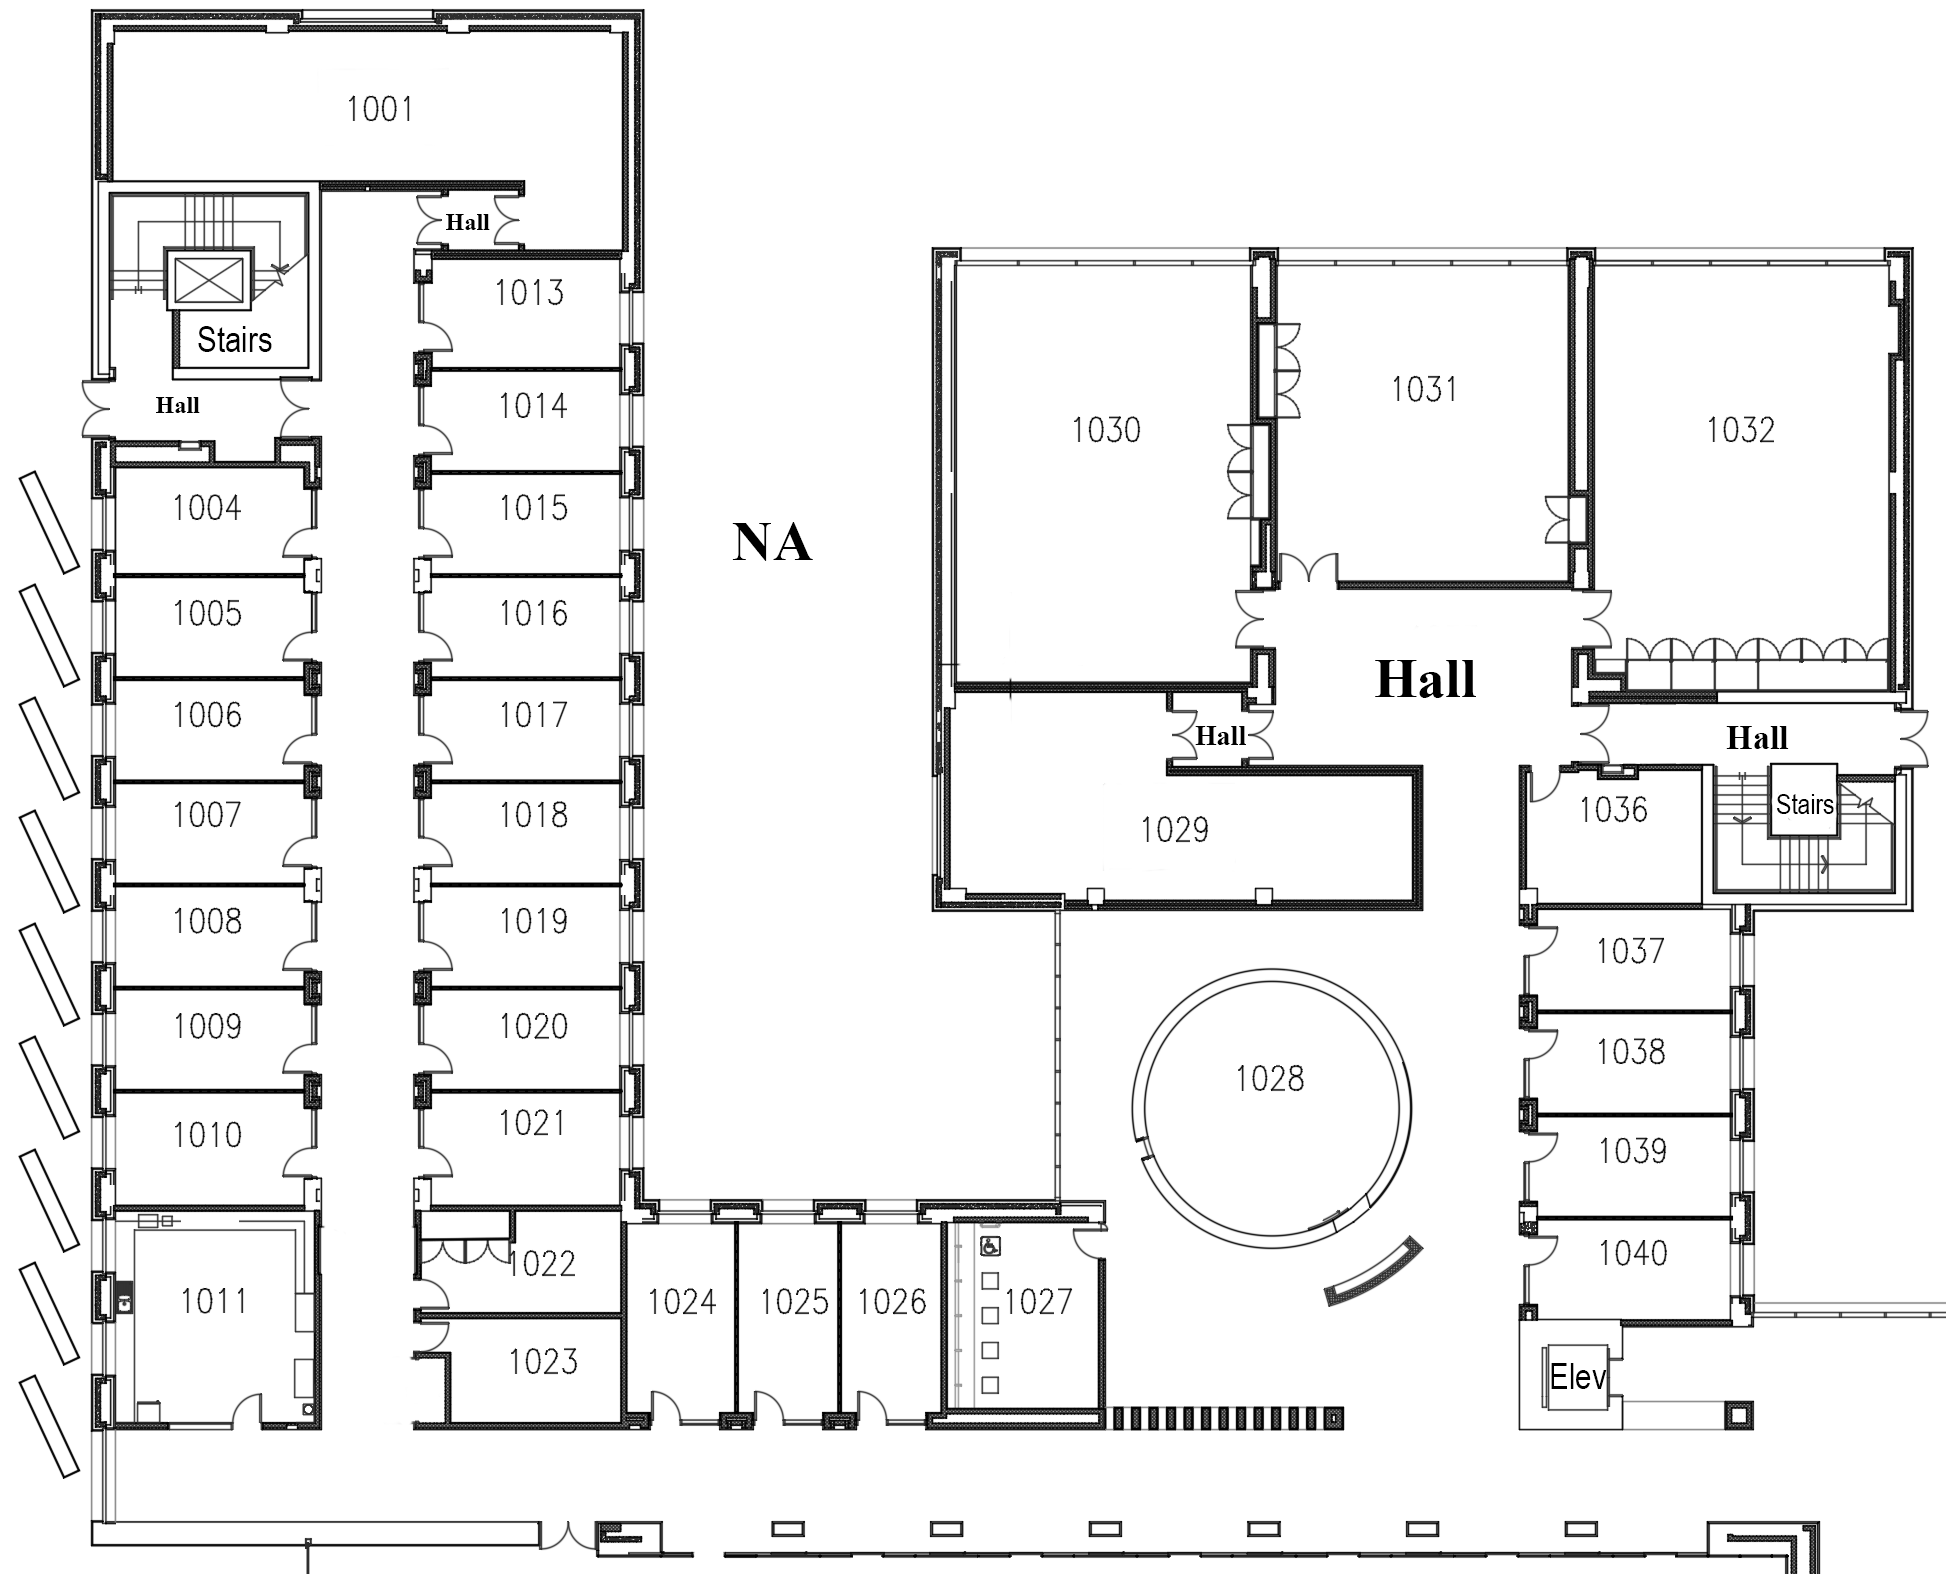
\includegraphics[width=\linewidth]{figures/dataset_ff.png}
\Description{Annotated first-floor drawing with room, hall, stairs, and elevator labels.}
\caption{First-floor section A.}
\end{subfigure}
\hfill
\begin{subfigure}{0.40\textwidth}
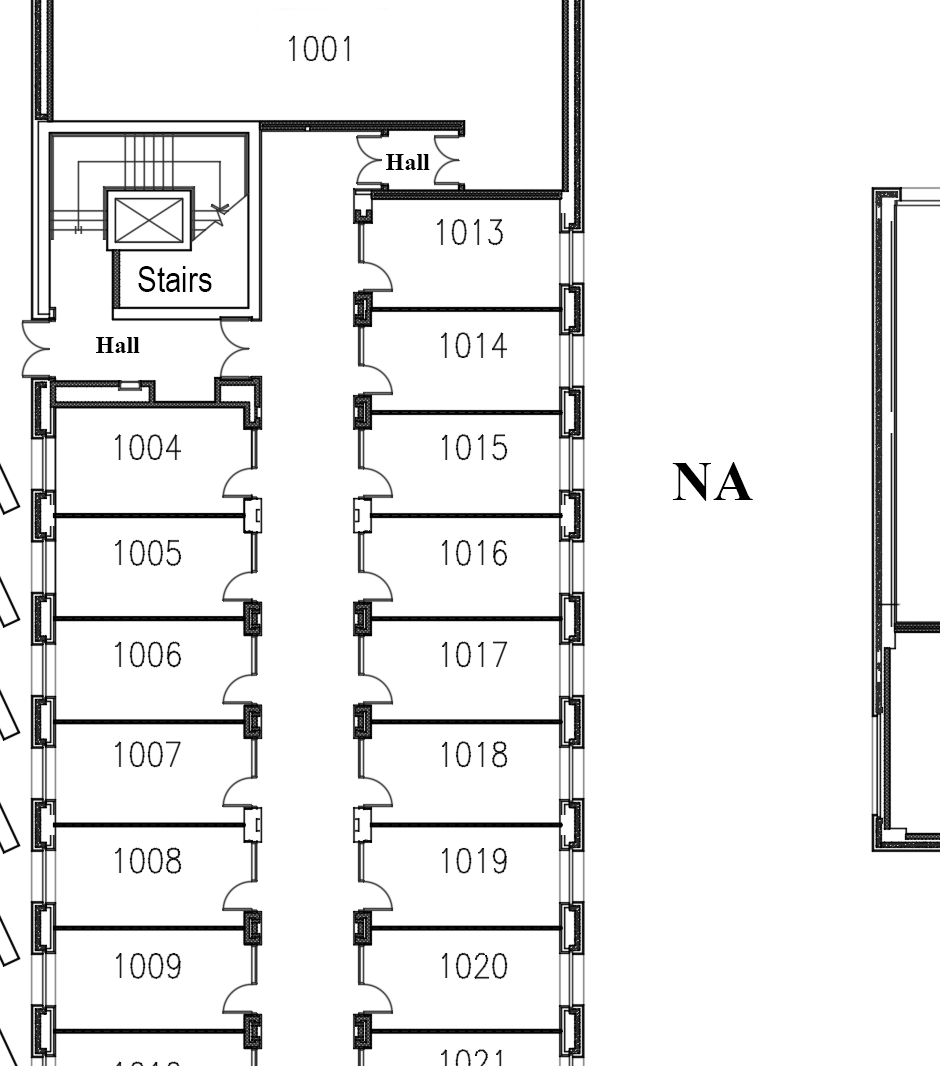
\includegraphics[width=\linewidth]{figures/dataset_ff_crop.png}
\Description{Enlarged detail of the drawing showing labels, door symbols, and walls.}
\caption{Detail view of the annotation conventions.}
\end{subfigure}
\Description{Two annotated evaluation floor plans.}
\caption{\rone{A representative evaluation drawing and a detail view. Rooms carry numeric labels, corridors carry hall labels, outdoor regions carry na labels, and stairs and elevators are labeled at their shafts. Walls are dark strokes and doors use standard arc symbols.}}
\label{fig:dataset}
\end{figure}

\begin{table}[!htbp]
\centering
\caption{\rall{Evaluation corpus. Room, exit, and transition counts refer to the post-pruning graphs.}}
\label{tab:dataset}
\begin{tabular}{lrrrr}
\toprule
Plan & Size (px) & Rooms & Exits & Transitions \\
\midrule
First-floor section A & $1946 \times 1574$ & 34 & 2 & 3 \\
First-floor section B & $1596 \times 1120$ & 35 & 10 & 0 \\
First-floor section C & $1122 \times 1126$ & 28 & 3 & 0 \\
First-floor section D & $1712 \times 1082$ & 20 & 2 & 0 \\
Ground-floor section & $1182 \times 1105$ & 3 & 0 & 3 \\
Ten smaller plans & various & 2--6 each & 0--6 each & 0 \\
\bottomrule
\end{tabular}
\end{table}

\subsection{Text and Semantics}
\label{subsec:text_eval}

\rone{Label detection is measured against a hand-enumerated ground truth of every label visible on the drawing. On first-floor section A the detector finds 43 of 43 labels, and recognition is exact for 41 of 43. Both failures truncate the leading digit of a room number, for example 1011 becomes 101. The consequences differ by failure class. A misrecognized numeric label still yields a valid room node with a wrong name, so connectivity is unaffected. A label missed entirely leaves its region without a semantic seed, and the region is not instantiated. An unlabeled variant of the same drawing demonstrates the extreme case by producing zero transition nodes and failing the five-class requirement of door classification.}

\rone{Label placement supports the main-node choice. Across 172 rooms on nine sections, the label sits a median of 0.24 room-equivalent radii from the geometric centroid of its region, with a mean of 0.27 and a worst case of 0.98, and 92\% of labels fall inside the room's inscribed circle. Architectural drafting practice places labels centrally, so seeding main nodes at labels is empirically sound.}

\subsection{Connectivity under Door-Detector Degradation}
\label{subsec:degradation}

\rall{Door detection is the dominant failure source, so we quantify how detector errors propagate to connectivity. The experiment deletes doors from the pre-pruning graph, where the full corridor and room mesh is intact, and measures pairwise room completeness and exit reachability with 20 Monte-Carlo draws per level. Deletions apply to the detector output because no door-level ground truth exists for these drawings, so the curves measure sensitivity relative to the current detector. Figure~\ref{fig:knockout} shows the curves for random deletion and for deletion restricted to room-to-corridor and corridor-to-corridor doors.}

\begin{figure}[!htbp]
\centering

\includegraphics[width=\textwidth]{figures/knockout_curves.png}
\Description{Completeness and exit reachability curves under door deletion for three floor sections.}
\caption{\rall{Connectivity under door deletion for three floor sections. Random deletion and room-to-corridor deletion degrade completeness steadily because each room is single-homed through one access door. Corridor-to-corridor deletion barely moves two of the floors and bites on the third, which motivates the per-door analysis.}}
\label{fig:knockout}
\end{figure}

\rall{Per-door analysis sharpens the picture. Deleting each corridor-to-corridor door alone shows that most such doors are redundant because the corridor mesh reconnects around them. The exceptions are bridge doors whose removal disconnects entire sections. On first-floor section B a single such door costs 0.51 of completeness and 0.54 of exit reachability by itself. Bridge doors coincide with the cut vertices of the graph, so they are mechanically identifiable, which turns the dominant failure mode into a targeted verification problem. Section~\ref{sec:discussion} outlines the resulting repair direction.}

\subsection{Graph Quality, Ablations, and Pruning}
\label{subsec:graph_eval}

Graph quality is measured with an exhaustive metric layer. Completeness is the fraction of unordered main-room pairs connected by a path, exit reachability is the fraction of main rooms that reach at least one exit door, and both are computed from the full component structure rather than from samples. Most processed sections are fully connected. Three sections, among them section D of Table~\ref{tab:dataset}, are fragmented as built with completeness between 0.51 and 0.76, which quantifies the corridor-door failure mode on real output.

\paragraph{Funneling Ablation.}
\rone{Three intra-room connectivity strategies are compared on the same floors, namely dense wiring from every family node to every family door, funneling, and a single node per room.} Table~\ref{tab:funneling} reports the outcome. \rtwo{All variants achieve complete family-to-door connectivity, and they differ in cost and route quality. Funneling retains 167 intra-room edges against 1{,}869 for dense wiring on section A, at a route stretch of 7.2\% over the dense reference, while the single-node variant pays 13.5\% and forfeits intra-room spatial fidelity. A second floor yields exactly one intra-room edge per subnode, which matches Proposition~\ref{prop:funneling}.}

\begin{table}[!htbp]
\centering
\caption{\rtwo{Funneling ablation on first-floor section A. Route lengths are subnode-to-nearest-exit means, and stretch is relative to dense wiring.}}
\label{tab:funneling}
\begin{tabular}{lrrrrr}
\toprule
Variant & Nodes & Edges & Completeness & Route stretch & Query (ms) \\
\midrule
Dense wiring & 878 & 1{,}273 & 1.000 & 1.000 & 0.44 \\
Funneling & 878 & 1{,}118 & 1.000 & 1.072 & 0.40 \\
One node per room & 680 & 918 & 1.000 & 1.135 & 0.35 \\
\bottomrule
\end{tabular}
\end{table}

\paragraph{Pruning Ablation.}
\rtwo{Each pruning keep-term is load-bearing. Re-deriving the keep-set with individual terms disabled shows that dropping the transition term silently removes every transition from the pruned graph, and dropping the exit term removes every exit door. The full pruning pass removes 59\% of nodes and 82\% of edges at a measured route inflation of exactly zero, because kept paths are shortest paths by construction, while mean single-pair query time improves from 2.10 to 0.50 milliseconds.} Figure~\ref{fig:prune} illustrates the reduction. \rone{This conservative keep-set is intentionally redundant, and the measured outcome justifies it, since connectivity and route quality are fully preserved at a fraction of the graph size.}

\begin{figure}[!htbp]
\centering

\includegraphics[width=\textwidth]{figures/pruning_comparison.png}
\Description{Bar chart of node and edge counts before and after pruning.}
\caption{Pre-pruning and post-pruning graph sizes on the two-floor merge.}
\label{fig:prune}
\end{figure}

\subsection{Corridor Sampling Density}
\label{subsec:density_eval}

\rone{Corridor node density buys a safety margin rather than reachability. Rerunning the full pipeline at grid spacings from 20 to 80 pixels shows that a 60-pixel grid keeps the graph fully connected with room-to-exit routes within 4.6\% of the 20-pixel default at 57\% fewer nodes. At 80 pixels the corridor mesh fragments, completeness collapses to 0.49, and routes err by 163\%. The failure mode is a cliff rather than a slope, so the dense default guards against narrow corridors at a known cost.} Figure~\ref{fig:density} plots the trade-off.

\begin{figure}[!htbp]
\centering
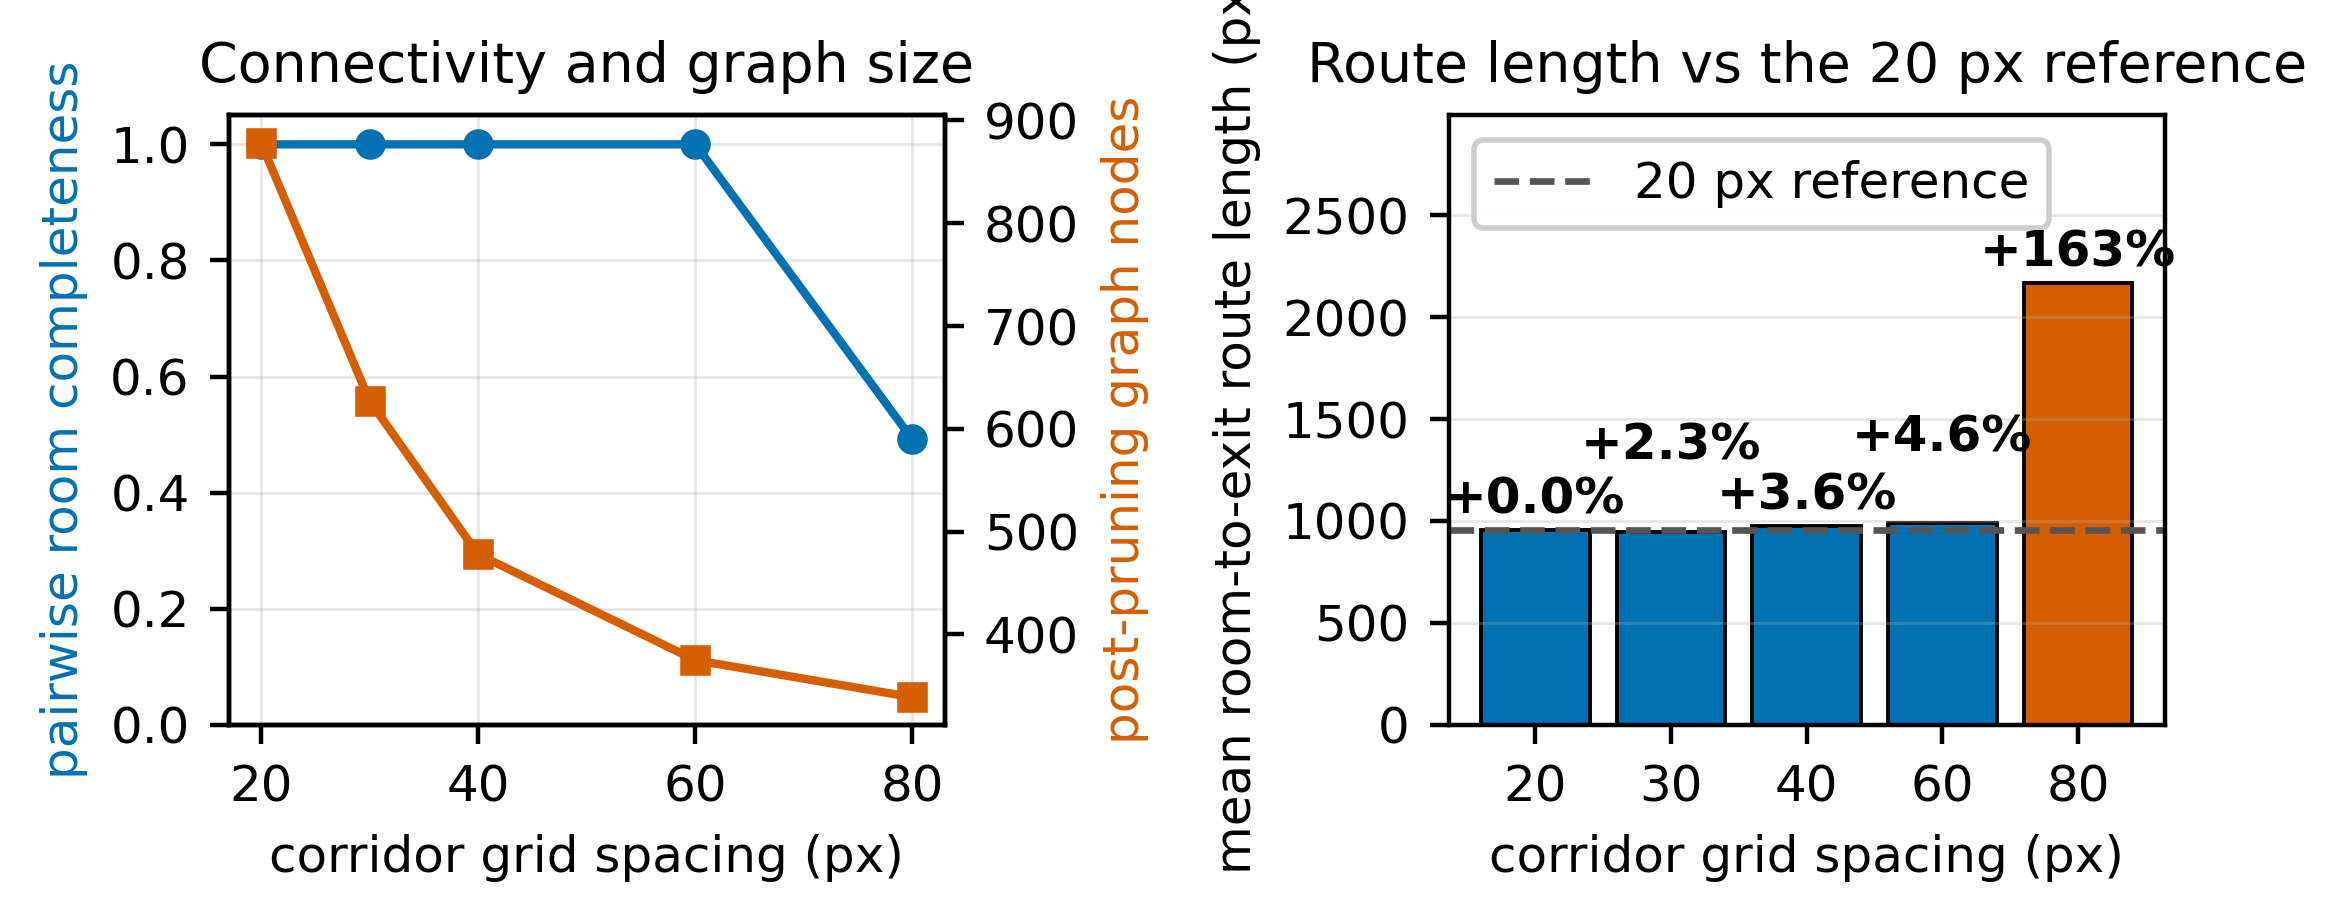
\includegraphics[width=\textwidth]{figures/corridor_density.png}
\Description{Completeness and node count as functions of corridor grid spacing.}
\caption{\rone{Corridor density trade-off on first-floor section A. The left panel shows that completeness holds from 20 to 60 pixels and collapses at 80, while graph size grows steeply toward dense spacing. The right panel shows the mean room-to-exit route length per spacing, and the label above each bar gives its change relative to the 20-pixel reference.}}
\label{fig:density}
\end{figure}

\subsection{Route Fidelity against Free-Space Geodesics}
\label{subsec:fidelity}

\rall{Route quality is validated against an objective walkable reference. The reference is the free-space geodesic, the exact shortest path through the drawing's non-wall pixels with doorways opened at detected door positions. Straight-line distance is a poor reference because walls force real detours, and the measured ratio of geodesic to Euclidean distance runs between 1.35 and 1.67 on average with a maximum of 3.3. We report the geodesic reference in two variants that bracket the truth, a permissive bound over all free space and a conservative bound that excludes the semantic outside class.}

\rall{Graph routes track the geodesics closely on enclosed sections. On first-floor section A the stretch of graph routes over geodesics has a mean of 1.047 and a ninetieth percentile of 1.093 under both bounds. On the more open section B the conservative bound gives a mean stretch of 1.24 while the permissive bound gives 2.30, and the gap between the bounds quantifies sparse outdoor routing as a concrete limitation.} Figure~\ref{fig:fidelity} shows a verification overlay.

\begin{figure}[!htbp]
\centering
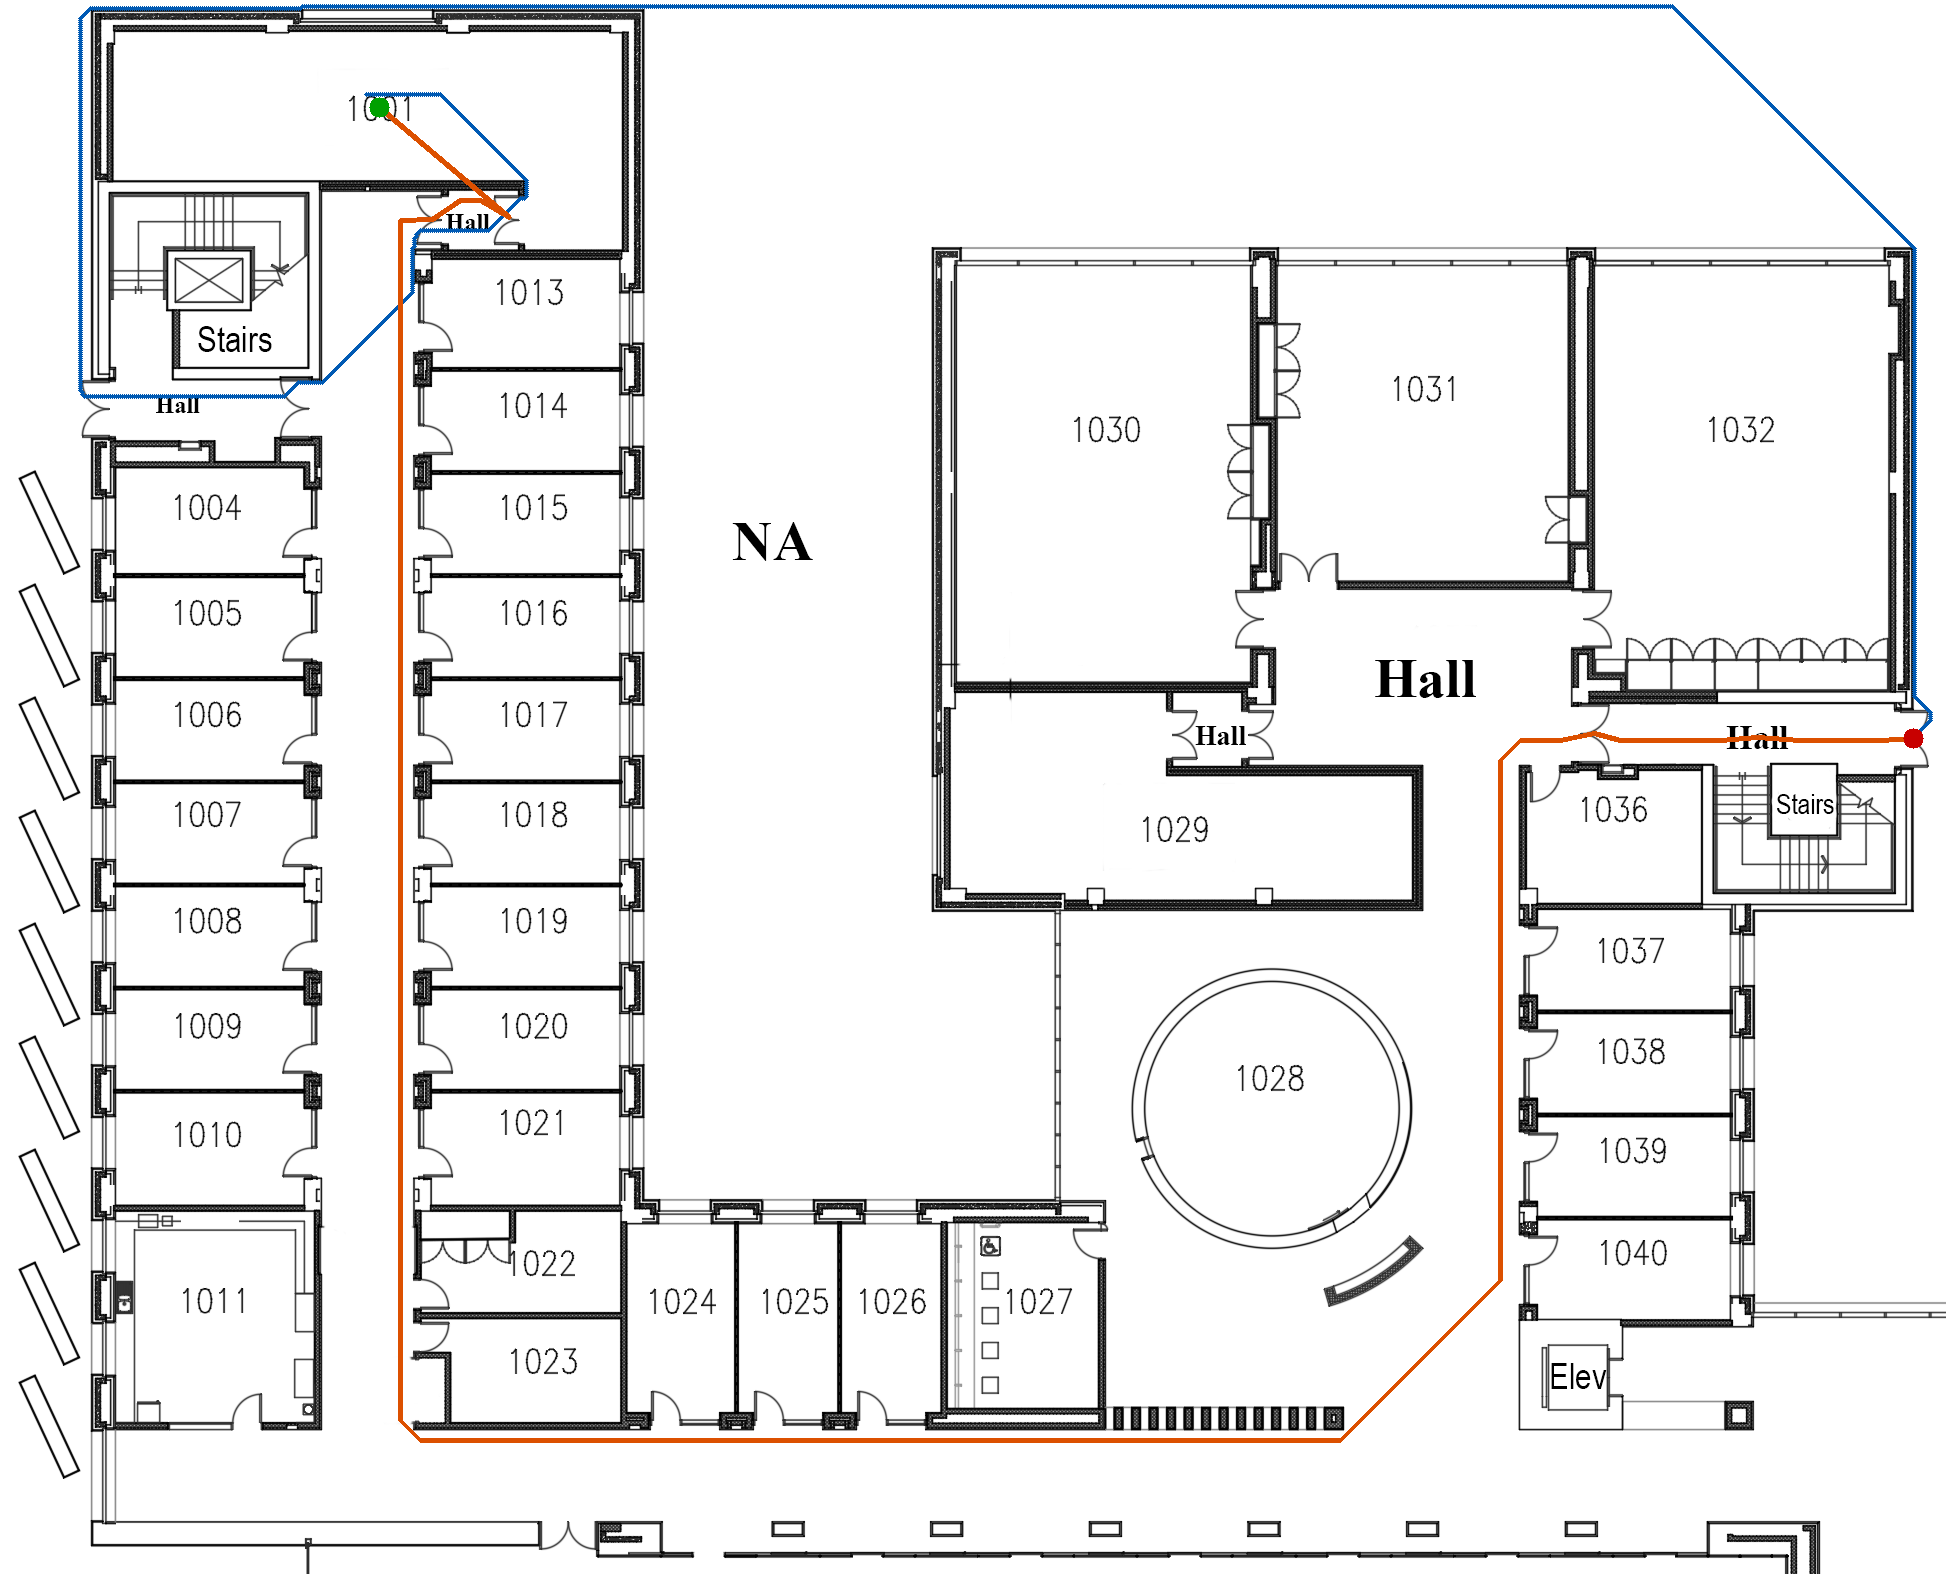
\includegraphics[width=0.7\textwidth]{figures/fidelity_overlay.png}
\Description{Floorplan overlay showing a free-space geodesic and the corresponding graph route.}
\caption{\rall{Verification overlay for one room-to-exit pair. The dotted trace is the free-space geodesic and the solid polyline is the graph route.}}
\label{fig:fidelity}
\end{figure}

\subsection{Baseline Comparison}
\label{subsec:baseline}

\rthree{A structure-only baseline isolates the value of the typed construction. The baseline skeletonizes free space into a medial-axis routing backbone and receives our own room and exit detections, so the comparison targets routing structure alone.} Table~\ref{tab:baseline} reports the outcome on the same room pairs and the same geodesic reference. \rthree{The skeleton needs between 3.7 and 12 times more nodes, fails completeness because it fragments at doorway gaps, produces worse route stretch, and answers queries between 37 and 94 times slower. It also expresses none of the typed downstream tasks, since it has no rooms, doors, or transitions as objects.}

\begin{table}[!htbp]
\centering
\caption{\rthree{Medial-axis baseline versus \tesseract{} on two sections. Stretch is against the interior geodesic reference.}}
\label{tab:baseline}
\begin{tabular}{llrrrrr}
\toprule
Section & Graph & Nodes & Edges & Completeness & Stretch & Query (ms) \\
\midrule
A & Skeleton & 3{,}248 & 2{,}029 & 0.829 & 1.233 & 14.2 \\
A & \tesseract{} & 878 & 1{,}118 & 1.000 & 1.047 & 0.38 \\
B & Skeleton & 8{,}598 & 6{,}959 & 0.782 & 1.381 & 34.0 \\
B & \tesseract{} & 712 & 928 & 1.000 & 1.231 & 0.36 \\
\bottomrule
\end{tabular}
\end{table}

\subsection{Multi-Floor Evaluation}
\label{subsec:multi_eval}

\paragraph{Matching Robustness.}
\rall{The automatic matcher is evaluated under controlled perturbations of a real floor. A synthetic counterpart floor is generated by a known similarity transform plus five pixels of position jitter, so correctness is exact by construction. Matching accuracy is 1.000 across every sweep, namely translations to 400 pixels, rotations to 30 degrees, scale changes from 0.7 to 1.4, twin-shaft separations down to 25 pixels, and shaft-deletion tests in which the deleted shaft's partner must remain unmatched. A greedy nearest-neighbor baseline degrades to 0.75 accuracy on close twins. Median registration recovery error is 0.5 pixels under translation, 4.4 under rotation, and 4.9 under scale.} Figure~\ref{fig:matcher} shows the accuracy panels and Figure~\ref{fig:regerr} the recovery envelope.

\begin{figure}[!htbp]
\centering
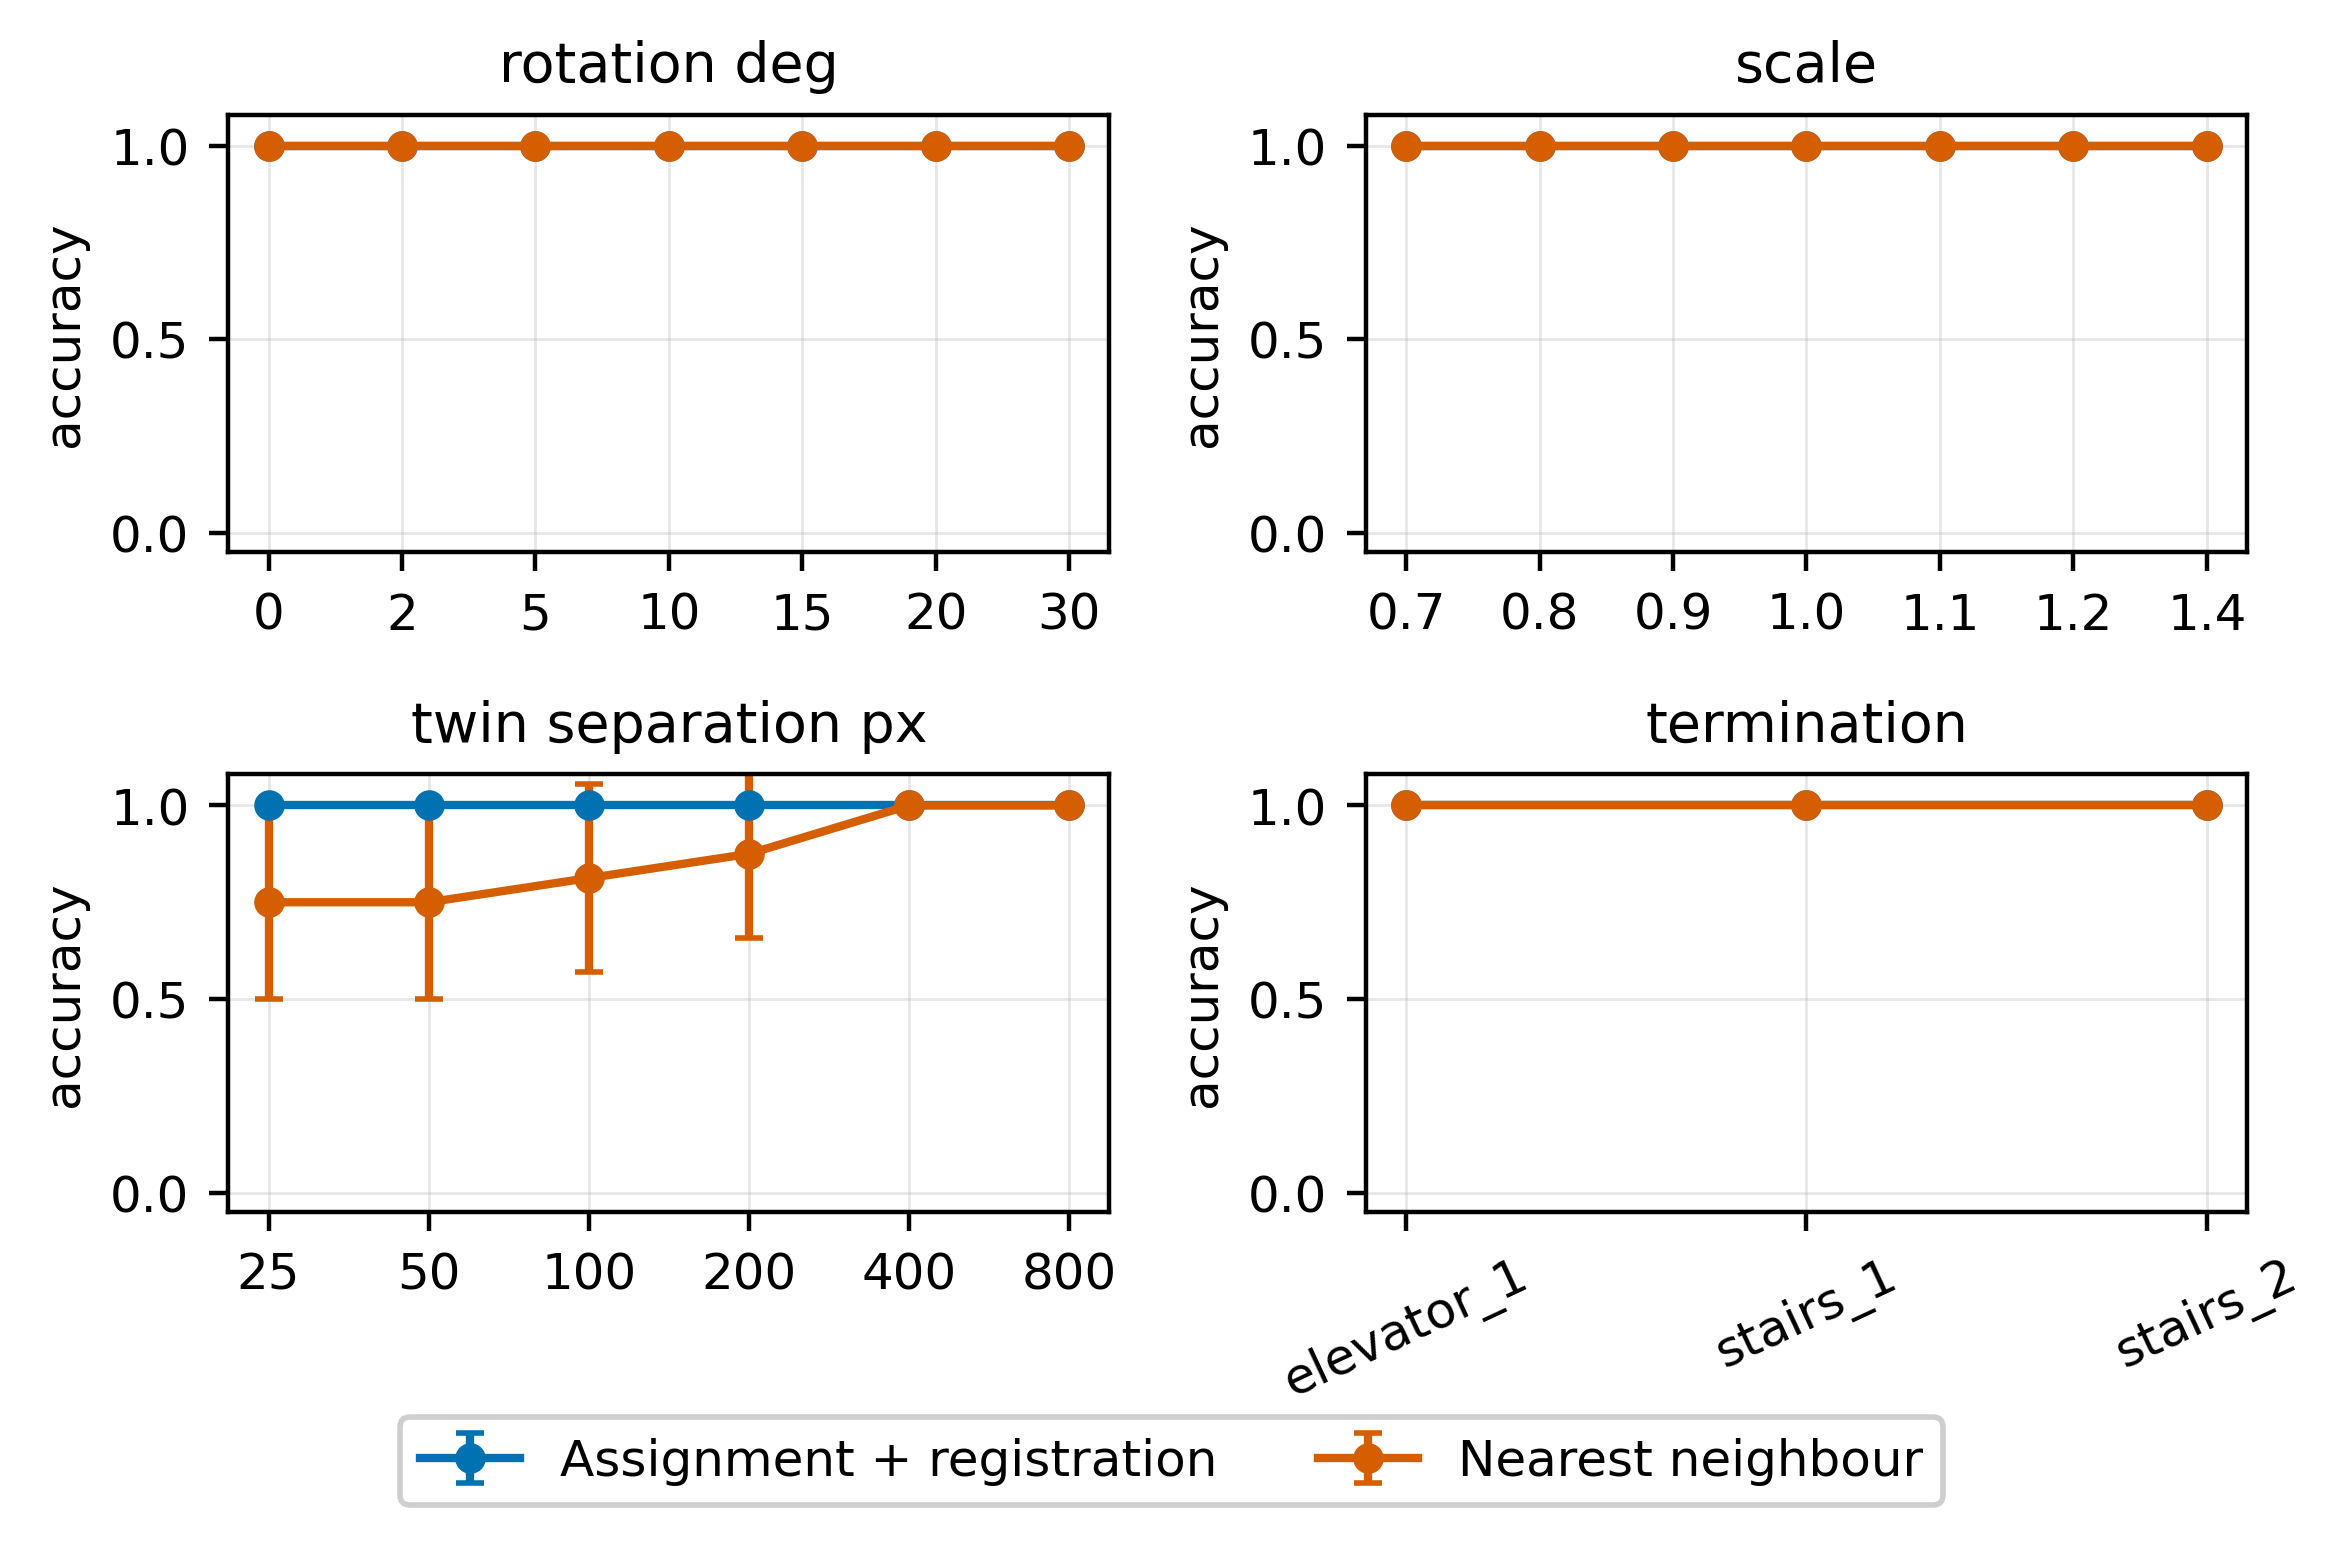
\includegraphics[width=\textwidth]{figures/matcher_eval.png}
\Description{Matching accuracy panels for five perturbation sweeps.}
\caption{\rall{Matching accuracy under synthetic perturbation for the rotation, scale, twin-separation, and shaft-deletion sweeps. The assignment matcher holds 1.000 throughout while the nearest-neighbor baseline degrades as twin shafts approach. The translation sweep behaves identically, and its recovery error appears in Figure~\ref{fig:regerr}.}}
\label{fig:matcher}
\end{figure}

\begin{figure}[!htbp]
\centering
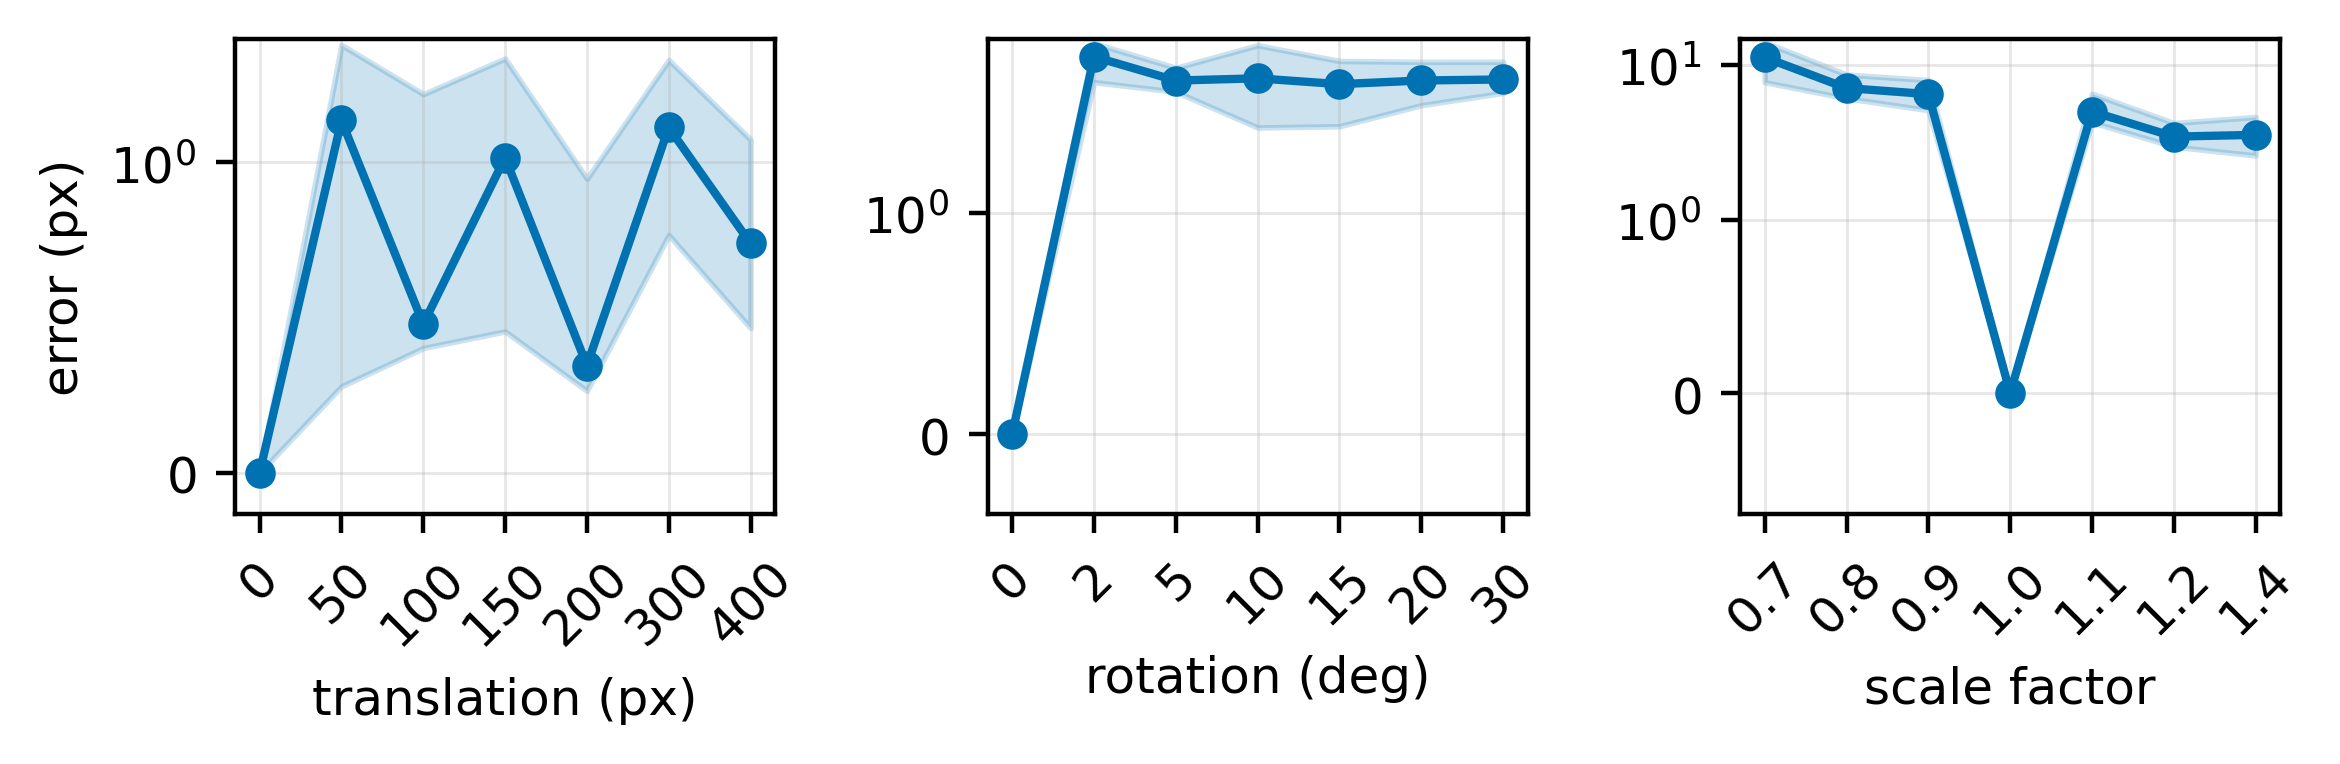
\includegraphics[width=\textwidth]{figures/registration_error.png}
\Description{Median registration recovery error with interquartile bands for three sweeps.}
\caption{\rall{Registration recovery error against known perturbations, shown as median with interquartile band.}}
\label{fig:regerr}
\end{figure}

\paragraph{Cross-Floor Case Study.}
\rall{A genuinely different floor pair exercises the conservative behavior. Matching the ground-floor section against the first-floor section, two drawings with different crops and extents, the door-width prior fixes the relative scale at 1.036, registration selects a single supported correspondence at a confidence of 0.83, and every remaining shaft on both floors is rejected rather than force-paired. The system flags the weak wall agreement and the single supporting pair in the mapping provenance, which is exactly the reviewable outcome intended for partially overlapping sections.}

\paragraph{Merged Graphs.}
The merged two-floor graphs are fully connected, and every room reaches every other room and at least one exit. \rthree{With modeled vertical travel weights the measured step-free detour ratio corrects from 2.02 to 1.79, which shows that nominal unit weights had inflated cross-floor route costs.}

\subsection{Downstream Task Validation}
\label{subsec:downstream}

\rone{Two navigation tasks validate the representation directly. Step-free routing forbids stairs and is expressible only because transitions are typed. On the two-floor merge with full transition correspondence, all 200 sampled cross-floor room pairs remain reachable without stairs, at a mean detour of 1.79 and a ninetieth percentile of 3.32 relative to unrestricted routing. On the ground-to-first-floor pair, where only a stairs correspondence is established, all 102 pairs are reachable normally and none is reachable step-free, which surfaces an accessibility gap that untyped graphs cannot express. Egress analysis computes each room's distance to its nearest exit by multi-source Dijkstra, and every room on the evaluation floors has an egress path with a median distance of 901 pixels and a ninetieth percentile of 1{,}503.}

\subsection{Timing}
\label{subsec:timing}

Table~\ref{tab:timing} reports the per-stage breakdown on first-floor section A.

\begin{table}[!htbp]
\centering
\caption{Single-floor processing time breakdown for a $1946 \times 1574$ drawing.}
\label{tab:timing}
\begin{tabular}{lr}
\toprule
Stage & Time (s) \\
\midrule
Text detection & 3.0 \\
Text interpretation & 2.5 \\
Flood-fill segmentation & 9.0 \\
Door detection & 21.2 \\
Door classification & 2.9 \\
Node updates and entry doors & 4.8 \\
Edge creation & 0.1 \\
Pruning & 2.0 \\
\midrule
\textbf{Total} & \textbf{52.0} \\
\bottomrule
\end{tabular}
\end{table}

\subsection{Qualitative Results}
\label{subsec:qualitative}

Figure~\ref{fig:stacked} visualizes a merged two-floor graph with its inter-floor connections.

\begin{figure}[!htbp]
\centering

\includegraphics[width=\textwidth]{figures/stacked_floors.png}
\Description{Stacked visualization of a merged two-floor graph with inter-floor links.}
\caption{Side-by-side visualization of a merged two-floor graph. Star markers in matching colors identify the matched transition shafts on each floor.}
\label{fig:stacked}
\end{figure}

% ==============================================================================
% 11. DISCUSSION
% ==============================================================================
\section{Discussion and Limitations}
\label{sec:discussion}

\paragraph{Operating Envelope.}
\rthree{The system targets drawings that satisfy the conventions of Section~\ref{subsec:input}. Hand-drawn sketches, sparsely annotated plans, non-standard door symbols, and drawings whose walls cannot be recovered by thresholding fall outside the envelope. A missing label class causes rejection rather than silent mis-segmentation, which we consider the safer failure.}

\paragraph{Door Detection and Repair.}
\rall{Missed corridor doors remain the dominant threat to connectivity, and the degradation study shows the damage concentrates in bridge doors that coincide with graph cut vertices. This observation yields a concrete repair direction, namely verifying the wall image along candidate bridges between disconnected components and inserting flagged doors where a door-width opening exists. We scope this image-guided repair as immediate future work rather than claiming it here.}

\paragraph{Directional Constraints.}
\rtwo{The graph is undirected, so one-way doors and emergency-only egress are not modeled. Directional edge attributes are a natural extension.}

\paragraph{Registration and Matching.}
\rall{Automatic matching depends on registration evidence. Partially overlapping sections yield weak wall agreement, mirrored drawings are detected and flagged rather than corrected silently, and floors that share fewer than two true correspondences rely on the door-width scale prior. The system reports these conditions as explicit warnings, and a hand-written mapping remains the override for cases the evidence cannot settle.}

\paragraph{Outdoor Routing.}
\rall{The gap between the permissive and conservative fidelity bounds on open sections shows that outdoor routing is sparser than indoor routing. Denser outdoor sampling would narrow this gap at a known node cost.}

\paragraph{Computational Requirements.}
Neural network inference dominates processing time. GPU acceleration would reduce latency for deployment scenarios.

\paragraph{Ground Truth Availability.}
Quantitative evaluation remains limited by the absence of standardized floorplan-to-graph benchmarks. The free-space geodesic reference reduces this dependency for route quality, and we encourage community development of annotated datasets for full-graph comparison.

% ==============================================================================
% 12. CONCLUSION
% ==============================================================================
\section{Conclusion}
\label{sec:conclusion}

We presented \tesseract{}, an end-to-end system that extracts navigable graph representations from annotated building floorplans. The pipeline integrates text detection, semantic interpretation, spatial segmentation, door detection, and typed graph construction, and it extends to multi-floor buildings through automatic transition matching and validated merging.

The revision establishes four main results. \rone{Room-family funneling carries a proven guarantee of complete intra-room connectivity at linear intra-room edge cost, and an ablation places it at the size-quality sweet spot.} \rall{Vertical correspondences are inferred automatically through registration and assignment with rejection, with perfect accuracy under controlled perturbation and conservative, warning-guarded behavior on partially overlapping real sections.} \rall{Graph routes stay within 4.7\% of exact free-space geodesics on the primary evaluation floor, and pruning removes 59\% of nodes and 82\% of edges at zero measured route cost.} \rthree{A structure-only medial-axis baseline confirms that the typed construction wins on size, completeness, route quality, and query time simultaneously.}

Future work includes image-guided repair of bridge doors, extension to non-annotated floorplans through learned segmentation, directional edge attributes, and standardized benchmarks for floorplan-to-graph evaluation.

% ==============================================================================
% ACKNOWLEDGMENTS
% ==============================================================================
\begin{acks}
% [FILL: Funding acknowledgments, contributor credits]
\end{acks}

% ==============================================================================
% BIBLIOGRAPHY
% ==============================================================================
\bibliographystyle{ACM-Reference-Format}
\bibliography{bibliography}

% ==============================================================================
% APPENDIX
% ==============================================================================
\appendix

\section{Implementation Details}
\label{app:implementation}

\subsection{Pipeline Parameters}
The wall threshold is 240 on the grayscale intensity. Room subnodes use hexagonal spacing of 60 pixels with a 10-pixel wall padding and 4-pixel jitter. Corridor sampling defaults to a 20-pixel grid, configurable per run. Outdoor sampling uses a 40-pixel grid.

\subsection{Matching Parameters}
Wall masks for registration are downsampled to 400 pixels on the long side, and connected components below 30 square pixels are removed as glyphs. Alignment counts a pair within 2\% of the image diagonal. Plausibility gates accept scales between 0.4 and 2.5 and rotations up to 60 degrees, and chamfer scoring requires at least 25\% mutual coverage. The rejection price is 0.10, and the cost weights are 1.0 for position, 1.0 for kind mismatch, and 0.05 for graph context. Inter-floor weights use a 0.9-meter door leaf, a 4-meter story height, and travel factors of 2.2 for stairs and 1.0 for elevators.

\section{Additional Visualizations}
\label{app:visualizations}

Figures~\ref{fig:app_ff} and~\ref{fig:app_gf} reproduce the two evaluation drawings at full page width so that labels, door symbols, and wall conventions are legible.

\begin{figure}[!htbp]
\centering
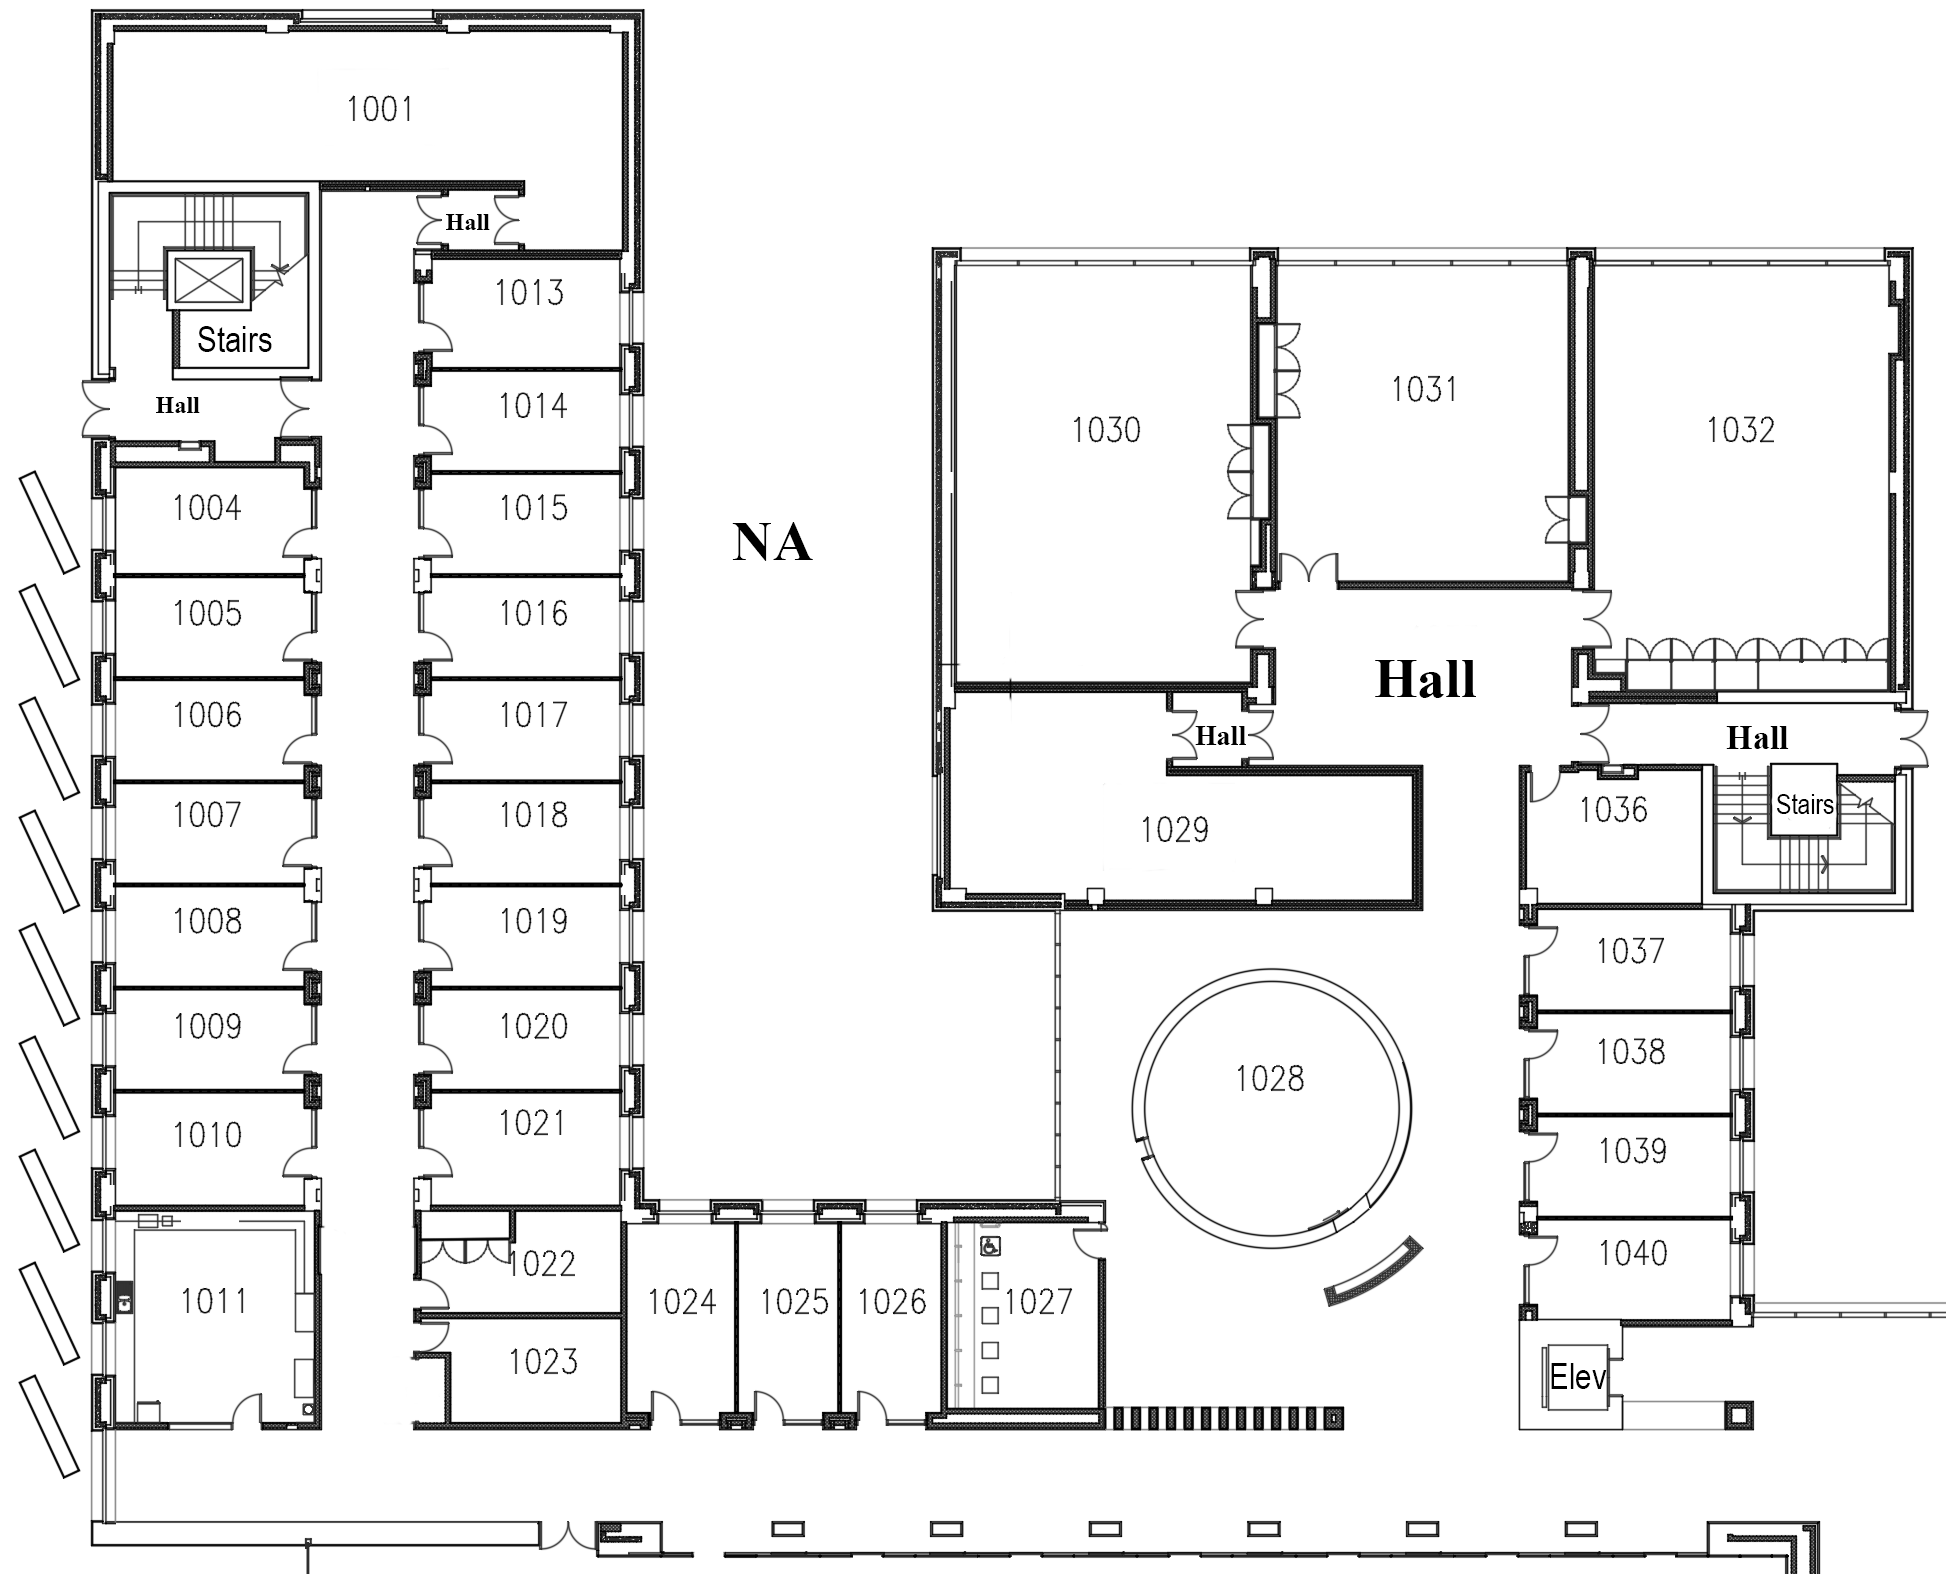
\includegraphics[width=\textwidth]{figures/dataset_ff.png}
\Description{Annotated first-floor drawing with room, hall, stairs, and elevator labels.}
\caption{First-floor section A at full width.}
\label{fig:app_ff}
\end{figure}

\begin{figure}[!htbp]
\centering
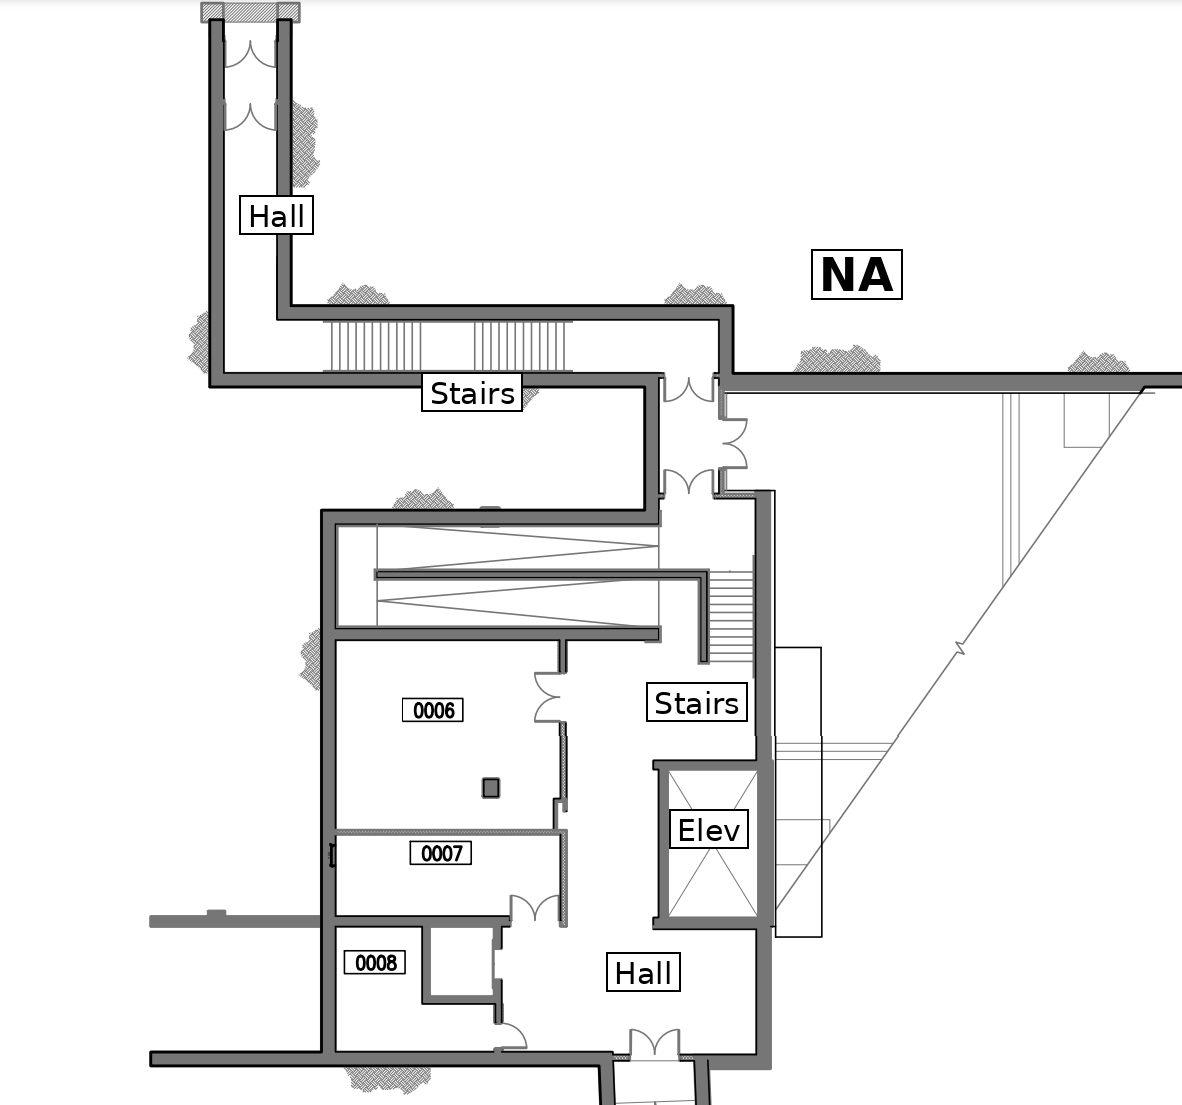
\includegraphics[width=0.85\textwidth]{figures/dataset_gf.png}
\Description{Annotated ground-floor drawing with room, hall, stairs, and elevator labels.}
\caption{Ground-floor section at full width.}
\label{fig:app_gf}
\end{figure}

\section{JSON Schema}
\label{app:schema}

Exported graphs contain a node list and an edge list. Nodes carry \texttt{id}, \texttt{type}, \texttt{position}, \texttt{floor}, and \texttt{pixels}, with room nodes adding \texttt{is\_subnode}, \texttt{parent\_room\_id}, area statistics, and anchor-door references, and door nodes adding subtype and connectivity references. Edges carry \texttt{source}, \texttt{target}, \texttt{weight}, \texttt{distance}, and \texttt{edge\_type}. Merged graphs add \texttt{original\_id} and \texttt{source\_image} per node.

\end{document}
